% thesis.tex
%
% This file is root file for an example thesis written using the
% University of Wisconsin-Madison LaTeX Style file.
%
% It is provided without warranty on an AS IS basis.


%=====================================================================
% Document Style
%=====================================================================
% Choose only one of the following document classes:
%
% for a 12 Point UW PhD Thesis without Margin Check
% \documentclass[12pt]{withesis}
%
% for a 10 Point UW PhD Thesis with Margin Check
%\documentclass[10pt,margincheck]{withesis}
%
% The margincheck option flags lines which overflow their hbox with a black
%  box at the end of the line.  This usually (but not always) indicates a
%  margin violation on the right margin.  Left margin violations aren't
%  indicated and if the margin violation is large enough, there isn't room
%  for the black box to be visiable.
%
% This option can be also used in conjunction with the msthesis option.
%
% or for a 12 Point UW Masters Thesis
\documentclass[12pt,msthesis]{withesis}
%
% or for a 10 Point UW Masters Thesis
%\documentclass[10pt,msthesis]{withesis}
%
% The msthesis option changes the page margins from 1" all around
% (the PhD format) to 1.25" left and 1" remaining margins (MS format).
% The defaults for degree and thesis are changed to be MS and thesis.
% These defaults can be overridden if the margins for the MS thesis
% are desired for other documents.

% To include optional packages, use the \usepackage command.
%  The package epsfig is used to bring in the Encapsulated PostScript
%    figures into the document.
%  The package times is used to change the fonts to Times Roman; however
%    because the times typewriter font looks odd, the original LaTeX
%    Computer Modern font is kept for the typewriter font using
%      \renewcommand{\ttdefault}{cmtt}
%    Note that Times Roman is a PostScript font and therefore, the document
%    cannot be correctly viewed from the *.dvi file.  It should be converted
%    to a *.ps file first and then viewed with a PostScript previewer...
\usepackage{epsfig}
\usepackage{times}
\usepackage{helvet}
\usepackage{courier}
\usepackage{multirow}
\usepackage{url}
\usepackage{algorithm}
\usepackage{algorithmic}
\usepackage{graphicx}
\usepackage{subfigure}
\usepackage{amssymb}
\usepackage{listings}

\renewcommand{\ttdefault}{cmtt}
\lstset{breaklines=true}
\renewcommand{\topfraction}{0.9}	% max fraction of floats at top
    \renewcommand{\bottomfraction}{0.8}	% max fraction of floats at bottom
    %   Parameters for TEXT pages (not float pages):
    \setcounter{topnumber}{2}
    \setcounter{bottomnumber}{2}
    \setcounter{totalnumber}{4}     % 2 may work better
    \setcounter{dbltopnumber}{2}    % for 2-column pages
    \renewcommand{\dbltopfraction}{0.9}	% fit big float above 2-col. text
    \renewcommand{\textfraction}{0.07}	% allow minimal text w. figs
    %   Parameters for FLOAT pages (not text pages):
    \renewcommand{\floatpagefraction}{0.7}	% require fuller float pages
	% N.B.: floatpagefraction MUST be less than topfraction !!
    \renewcommand{\dblfloatpagefraction}{0.7}	% require fuller float pages
    \renewcommand{\algorithmicrequire}{\textbf{Input:}}
    \renewcommand{\algorithmicensure}{\textbf{Output:}}
%========================================================================
%  Draft Control Commands:
%========================================================================
%
% \psdraft causes the \psfig or \epsfig commands to draw a box and label
% the box with the postscript file name instead of reading in the full
% postscript figure.  This can save time and toner when printing drafts.
%
%\psdraft
%
%
% \psfull causes the inclusion of the postscript figures.
%\psfull
%
%
%\pagestyle{thesisdraft} causes the footer text to become:
% DRAFT: Do Not Distribute        <time><Date>        <input file name>
%
%\pagestyle{thesisdraft}
%
%\pagestyle{thesis} causes the header and footers to be the correct format
%
\pagestyle{thesis}
%
%
%  The page margins can be marked with a post-script box using the
%  \draftmargins command.  This command uses dvips's end-of-page hook
%  This is only visible in the *.ps file (NOT the *.dvi file)!
%
%\draftmargins
%
%
%  The word ``DRAFT'' can be diagonally printed across the page using
%  the \draftscreen command.  This command uses dvip's beginning-of-page
%  hook.  This is only visible in the *.ps file (NOT the *.dvi file)!
%	
%\draftscreen


%=======================================================================
% Remove the following lines if appendix tables or figures are present.
% The suppress writing the auxiliary information which appears in the
% list of tables or list of figures.
%
%\noappendixtables                % Don't have appendix tables
%\noappendixfigures               % Don't have appendix figures


%=======================================================================
% End of Preamble, start of document
%


\begin{document}

% Choose your bibliography style
% plain is the basic style, others include ieeetr, siam, asm, etc
\bibliographystyle{ieeetr}


% prelude.tex
%   - titlepage
%   - dedication
%   - acknowledgments
%   - table of contents, list of tables and list of figures
%   - nomenclature
%   - abstract
%============================================================================


\clearpage\pagenumbering{roman}  % This makes the page numbers Roman (i, ii, etc)



% TITLE PAGE
%   - define \title{} \author{} \date{}
\advisorname{Soumya Ray}
\advisortitle{Professor}
\title{A Decision Theoretic Approach to Natural Language Generation}
\author{Nathan McKinley}
\date{2013}
%   - The default degree is ``Doctor of Philosophy''
%     (unless the document style msthesis is specified
%      and then the default degree is ``Master of Science'')
%     Degree can be changed using the command \degree{}
\degree{Master of Science}
%   - The default is dissertation, unless the document style
%     msthesis was specified in which case it becomes thesis.
%     If msthesis is specified for the MS margins, you can
%     still have a dissertation if you specify \disseration
%\disseration
%   - for a masters project report, specify \project
%\project
%   - for a preliminary report, specify \prelim
%\prelim
%   - for a masters thesis, specify \thesis
\thesis
%   - The default department is ``Electrical Engineering''
%     The department can be changed using the command \department{}
\department{Electrical Engineering and Computer Science}
%   - once the above are defined, use \maketitle to generate the titlepage
\makeatletter
\renewcommand\@date{January, 2014}
\makeatother
\maketitle

\clearpage
\begin{center}
{\bf CASE WESTERN RESERVE UNIVERSITY
SCHOOL OF GRADUATE STUDIES}\\

We hereby approve the thesis of\\
NATHAN MCKINLEY\\
candidate for the Master of Science degree*.\\
\end{center}
\noindent
Dr. Soumya Ray\\
Dr. Michael Lewicki\\
Dr. Gregory Lee\\
Dr. Vincenzo Liberatore\\

\noindent
Date: December 2, 2013\\

\noindent
*We also certify that written approval has been obtained for any
proprietary material contained therein.

% COPYRIGHT PAGE
%   - To include a copyright page use \copyrightpage
\copyrightpage

% ACKNOWLEDGMENTS
\begin{acknowledgments}
I thank my advisor, Professor Soumya Ray, for his assistance through the entire process of
developing this idea and creating this thesis.  When I began this program I knew very
little of the process of research, but Professor Ray guided me through creating my first
prototype of this system and my first paper for submission to a conference.  From there,
we ended up here, with the submission of my thesis in order to obtain the degree of
Master of Science.  I am very thankful to him for all his help, edits, and guidance.
\end{acknowledgments}

% CONTENTS, TABLES, FIGURES
\tableofcontents
\listoffigures

% ABSTRACT
\begin{umiabstract}
  % abstract.tex
%
% This file has the abstract for the withesis style documentation
%
% Eric Benedict, Aug 2000
%
% It is provided without warranty on an AS IS basis.

\noindent       % Don't indent this paragraph.
  We study the problem of generating a single sentence which satisfies
  a communicative goal, given a grammar which specifies the language.
  We model the generation process as a Markov Decision Process (MDP),
  using a reward function which reflects that communicative goal.  We use
  probabilistic planning to solve the MDP and generate a sentence which
  satisfies the communicative goal.  We compare our approach to a current
  state-of-the-art generation system, and find that our system can generally
  match the state-of-the-art in both performance and generation quality, while
  offering generation capabilities that exceed those usually found in planning-based
  generators.
\end{umiabstract}


\clearpage\pagenumbering{arabic} % This makes the page numbers Arabic (1, 2, etc)
                % Title page, committee approval sheet, abstract, table of contents, etc

% text
\chapter{Introduction}
Artificial Intelligence (A.I.) systems are becoming increasingly prevalent in
modern consumer products.  Google's ``Google Now" system determines
what information its user wants to see before they ask for it.  Apple's ``Siri"
acts as an artificial personal assistant, attempting to respond to queries stated in
natural language.  Android (which includes Google Now) and iOS (which
includes Siri) have 85\% market penetration between them, and there are
over one billion smartphones active.

Visions of future A.I. systems have long included natural
language interfaces.  The ship's computer from Star Trek, the robots from
the works of Heinlein and Asimov, and the droids from Star Wars are
all capable of human speech, and even those which are not capable of dialogue
are able to receive orders verbally and respond in kind.  The creation
of an artificial intelligence like humans have been imagining for many years
requires as a precondition the creation of a system for understanding and
creating language.

Consequently, a crucial subcomponent of artificial intelligence is Natural Language Processing (NLP).
NLP studies the task of interacting with humans using languages which are inherently
complex and ambiguous (e.g. English).
In order to successfully communicate with people, a system which does natural
language processing will need to accept language as input
and translate it into a format that computers can work with.  Such a system will also
need to be able to translate from an internal meaning representation to natural language.
See Figure \ref{nlp-block} for a visual explanation of this process.

For example, consider a robotic concierge system which takes phone calls from users.
A system like this has been shown to be practical\cite{litman_njfun_2000}, so it serves
as a good example of an NLG interaction.  One possible interaction might be the following:

\begin{verbatim}
Computer:  How may I help you today?
User    :  I am looking for a place to eat dinner.
\end{verbatim}

Once the user has finished speaking, the computer system has a series of electrical signals on
a phone line which it will need to decode into human speech.  This is the first step
in the block diagram of Figure \ref{nlp-block}.  Current-generation speech recognition
software is highly reliable for most accents, so let us assume that this step proceeds without
error.  At this point, the computer system will need to attempt to understand the natural
language input of "I am looking for a place to eat dinner".  There are many approaches
to this problem, but the previously-mentioned concierge system was able to get by with
a simple keyword-searching approach.  Such an approach might look for the words "I",
"place", "eat", and "dinner", and determine that the speaker desires a listing of restaurants that
are open for dinner.  This is the "NLP Parsing" step of Figure \ref{nlp-block}.  The system would
then do some internal processing (e.g. database queries), which makes up the "Processing"
step.  The system may determine that it needs to respond to the user, perhaps to ask a
clarifying question to narrow the user's search.  This determination will be made in the
"Response Generation" block.  At this point, the system will have an internal representation
of the type of question it needs to ask which we call a "communicative goal".  That goal might
look something like the following:
\begin{verbatim}
question type: clarifying
question seeks: preferences
question regards: dinner type.
question language: English
\end{verbatim}

At this point, the computer system needs to translate that into a sentence in its output
language.  The process of going from this internal representation to text like
"What type of food do you typically enjoy for dinner?" is called Natural Language Generation,
and comprises the fifth block of the NLP process.  Finally, this generated text is conveyed to
the user by encoding it into the data that can travel over a telephone, using a text-to-speech
program.

As this example shows, even without the aforementioned lofty future goals,
the increasing frequency of natural language interfaces for consumer
products shows that natural language generation (NLG) is becoming more and more important
in the world.  Consequently, a consistent and reliable method for creating a natural
language generation system would be of value, especially if the system's
computational requirements were small enough that the system could be embedded
in consumer electronics.

\begin{figure}
\centering
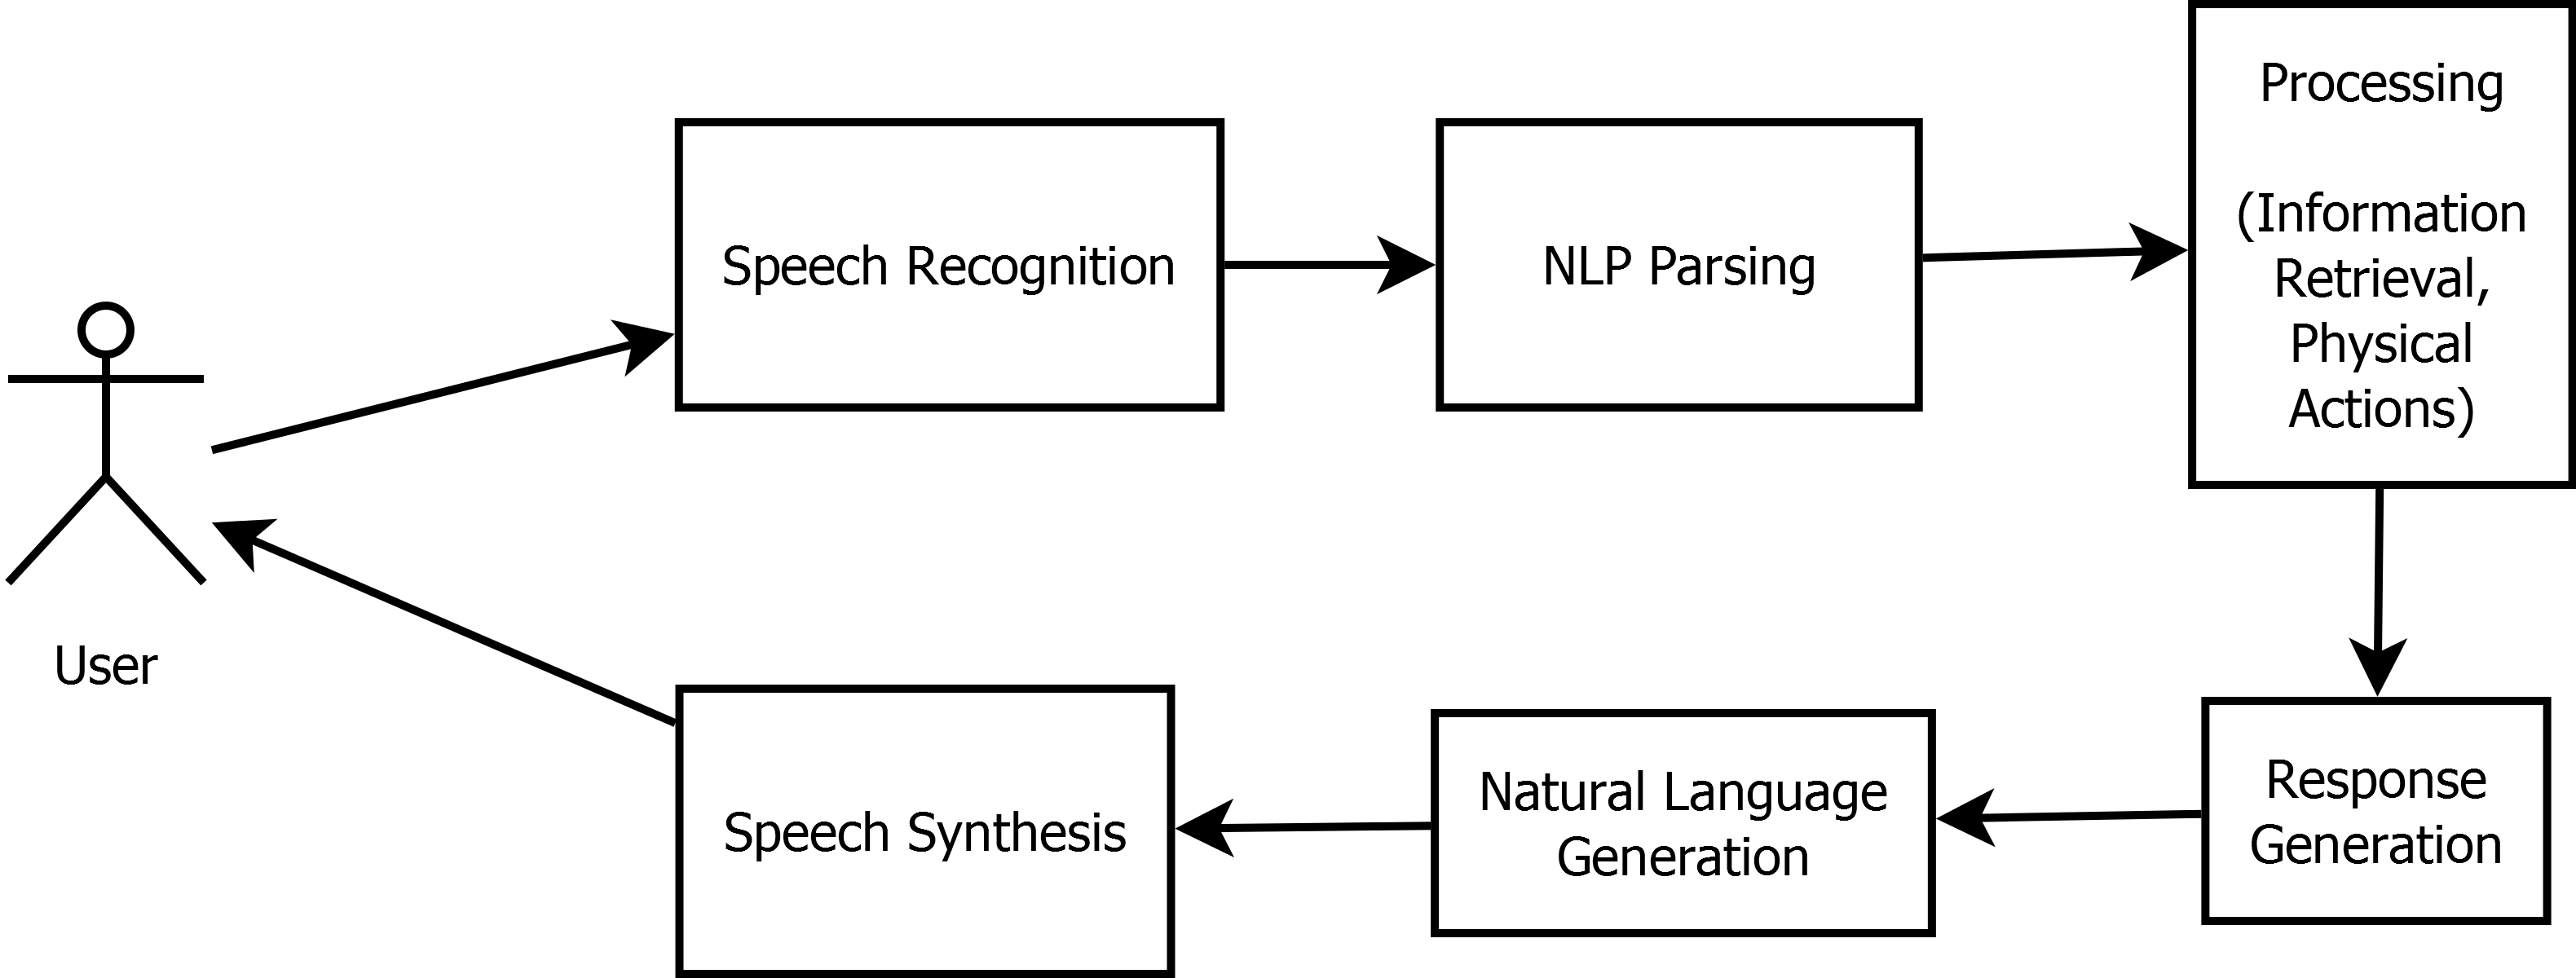
\includegraphics[width=0.8 \linewidth]{nlp-block.png}
\caption{A diagram showing the flow of information through a normal interaction
with a user in a generalized NLP system}
\label{nlp-block}
\end{figure}

In this thesis, we consider the following restricted NLG problem: given a
grammar, lexicon, and a communicative goal, output a valid English
sentence that satisfies this goal.  We call this problem "restricted", because
it assumes a level of knowledge about the context in which the generation
will occur.  In principle, the most general NLG problem is to produce a valid
sentence in an arbitrary language, using the entire grammar and lexicon available
in that language, to satisfy an arbitrary communicative goal.  In practice, we
rarely require this level of generality; it would be unnecessary for the concierge
program described above to be intimately familiar with the finer points of Klingon grammar.
In practice, therefore, our restricted problem is a reasonable one.

Previous work on this problem has taken two broad approaches.  On one hand we have
the classical planning approaches, which treat the problem of NLG as an AI planning
problem.  These systems have the advantage of being capable of finding acceptable
output in all circumstances where a perfect answer exists, but the disadvantage of
being unable to handle a probabilistic grammar in a structured way.  They also struggle
with completing a subset of the communicative goals, when full completion is not
possible.  On the other hand, there are statistical planners which work by examining the
most probable combinations of words and determining if any of those match the
meaning they are attempting to generate.  These have the advantage of completing
execution very quickly, and of taking advantage of Zipf's Law, which states broadly that
a very small subset of a language is used a very large proportion of the time.  They
have the disadvantage of requiring an inordinate amount of memory to be able to search
for the less-likely phrases and sentences which will occasionally need to be generated.
They also scale poorly with large grammar sizes.

We propose an algorithm which unifies these two approaches, and has, to some extent,
the advantages of both.  This algorithm gives
us the ability to efficiently search a large space (all possible natural language outputs) for 
one of many valid outputs.  We support probability in a structured way and allow
for generation using a large grammar.  We support partial completion of the communicative
goal, but strive for full completion when it is possible.  We allow for generation to stop
at any time and will return a partially-complete result very quickly.

We do this, broadly, by using probabilistic planning rather than classical planning.
Our algorithm is based in Monte-Carlo Tree Search, an increasingly
popular method for probabilistic planning.

We believe that if this algorithm were developed further, it could be useful as the
final step of a dialog system, or useful in generation situations where flexibility of the
generation system is crucial.  At present, it is already useful as the output stage of
a simple dialog system.  An efficient implementation would be able to take advantage
of multiprocessing and therefore run very well on a massively multiprocessing system,
enhancing performance substantially.

In chapter 2, we provide background information on NLG and probabilistic planning.  In chapter 3,
we discuss related work, including historical natural language generation frameworks.  We also
discuss the closest related system to ours, called CRISP.  In chapter 4, we present our framework
for natural language generation.  In chapter 5, we present our experimental evaluation of
our implementation, which shows that it performs comparably to the current state-of-the-art in
the field.  In chapter 6, we conclude by describing the potential applications and future work
using this method of generation.
\chapter{Background}
In this chapter, we provide some background on the algorithms
and underlying formalism which we build on in this work.  We explain
Markov Decision Processes, classical AI planning, probabilistic planning,
natural language grammars, and Monte Carlo Tree Search, each of which
is an important component in our algorithm.

\section{Markov Decision Processes}
A Markov Decision Process (MDP)~\cite{puterman_1994_markov}
is a tuple $(S, A, T, R, \gamma)$ where $S$ is a
set of states, $A$ is a set of actions available to an agent,
$T:S\times A\times S \rightarrow (0,1)$ is a possibly stochastic
function defining the probability $T(s,a,s')$ with which the
environment transitions to $s'$ when the agent does $a$ in state $s$.
$R:S\times A \rightarrow \mathbb{R}$ is a real-valued reward function that
specifies the utility of performing action $a$ in state $s$. Finally,
$\gamma$ is a discount factor that allows planning over infinite
horizons to converge. In such an MDP, the agent selects actions at
each state (a {\em policy}) to optimize the expected long-term
discounted reward: $\pi^*(s)=\arg \max_a E(\sum_t \gamma^t
R(s_t,a_t)|s=s_0)$, where the expectation is taken with respect to the
state transition distribution.

When the MDP model ($T$ and $R$) is
known, various dynamic programming algorithms such as value
iteration~\cite{bellman_1957_dynamic} can be used to plan and act in an MDP. When the
model is unknown, and the task is to formulate a policy, it can be
solved in a model-free way (i.e. without estimating $T$ and $R$)
through temporal difference (TD) learning. The key idea in TD-learning
is to take advantage of Monte Carlo sampling; since the agent visits
states and transitions with a frequency governed by the unknown
underlying $T$, simply keeping track of average rewards over time
yields the expected values required to compute the optimal actions at
each state.


\section{Planning}
Given a model of the world, an initial state and a goal state,
planning is the problem of finding a sequence of actions that gets us 
from the initial state to the goal state.
Depending on the environment, actions may be drawn from some distribution
dependent on the state of the world in which planning is being done.  This
state may be observable, partially observable, or invisible to the agent doing
the planning.  The actions that the agent takes usually transform the state of
the world in some way, and the goal is defined in terms of the state of the
world.

\subsection{Classical Planning}
Classical planning is a planning problem with six conditions.  In a classical planning problem,
there is a single initial state, which is fully known.  Actions are deterministic, can only
be taken by the single agent which is present in the world, and take unit time.  These three
conditions combine to mean that the world does not change without the agent causing the change.
The goal is one or more states which are reachable from the initial state, and
Finally, actions are sequential.

Classical planning has been studied extensively.  These problems are usually solved by two broad categories of
planning system: state-space planners and plan-space planners.  Forward state space planners
plan by taking actions from the initial state and examining the state that results from the action.  Since
actions are deterministic, it is straightforward to see that such a planner would be guaranteed to find
the goal state by trying every possible combination of actions.  Backward planners plan by working
backwards from the goal: they maintain a frontier and iteratively check which states in the state space
can reach the states in the frontier.

Plan-space planners work differently.  For state-space planners, every node in the planning graph
represents a state of the environment, reached through some list of ordered actions.  For plan-space
planners, each node in the planning graph represents a partial plan, not necessarily ordered.  These partial plans
have preconditions and effects; the plan is complete and correct when a node's effects are a superset
of the goal state and the same node's preconditions are a subset of the initial state.  Plan-space
planners begin with a node which has the entire goal state as its effects and its preconditions, then
iteratively refine the plan so that the preconditions become a subset of the initial state.

This iterative refinement is done in two ways: resolving open goals and resolving threats.
Open goals are preconditions of the plan which we have not yet resolved, and threats are
actions which are part of the plan whose effects cancel out the
preconditions of other actions which are part of the plan.  We resolve open goals by finding
actions whose effects contain the preconditions we seek to establish, then adding them to
the plan.  We resolve threats by introducing ordering constraints; the action which will
eliminate a necessary precondition should happen either before that precondition is established
or after the action which required it.

Plan-space planners can be faster than state-space planners at determining that a plan will be
impossible if some open goals cannot be resolved, but they can also be much slower if
continuing to resolve threats causes the plan to balloon in size.  In some domains, one
failure mode is substantially more likely than the other, and so a choice between the
two types of planners might be motivated by domain knowledge.

One popular plan-space planning algorithm is Graphplan\cite{graphplan}.  Graphplan works by creating
a "planning graph" which contains two types of nodes and three types of edges.  The two node types are
either representing facts in the world or representing actions which can be taken in the world.  The three edge
types are between a fact node and an action node, between an action node and a fact node, and between two
nodes of the same type.  Edges from a fact node to an action node represent preconditions (that action can be
taken if that fact is either true or false), and edges from an action node to a fact node represent effects (that
fact becomes true or false when the action is taken).  Edges from a node to a node of the same type represent
mutual incompatibility; two facts which cannot be true at the same time or two actions which cannot be taken
simultaneously (due to altering facts which are required preconditions, for instance).

Graphplan constructs this graph one level at a time, starting from the goal and working towards a state in which
all the facts which are true in the initial state are true in the graph.  It then works backwards by picking actions
that will reach the goal state from the initial state.  This may fail, and in that case the graph will be extended
another level and the search will be continued.  If the algorithm ever reaches a point where two successive
layers are identical, the algorithm will be terminated as a failure.



\subsection{Probabilistic Planning and the UCT algorithm}

Probabilistic planning is an alternative to Classical Planning when the preconditions required to solve the
easier problem do not hold.  Probabilistic planning (PP) is done on an MDP, where actions are not required
to be deterministic and where we attempt to maximize a reward function.  PP does require
full observability of the state (this was irrelevant during the classical planning
problem, since exploration with deterministic actions is trivial).  PP is often described
as determining a policy given a current state, rather than generating an ordered list of actions to take.

Determining the optimal policy at {\em every} state using the TD
strategy described in the above MDP discussion is polynomial in the size of the state-action
space~\cite{brafman_2003_rmax}, which is often intractable.
But for many applications, we do not
need to find the optimal policy in all states; rather we just need to {\em plan} in
an MDP from an initial state to achieve a single communicative goal. New techniques such
as sparse sampling~\cite{kearns_1999_sparse} and
UCT~\cite{kocsis_bandit_2006} show how to generate near-optimal plans
in large MDPs with a time complexity that is independent of the state
space size.

\begin{figure}
\centering
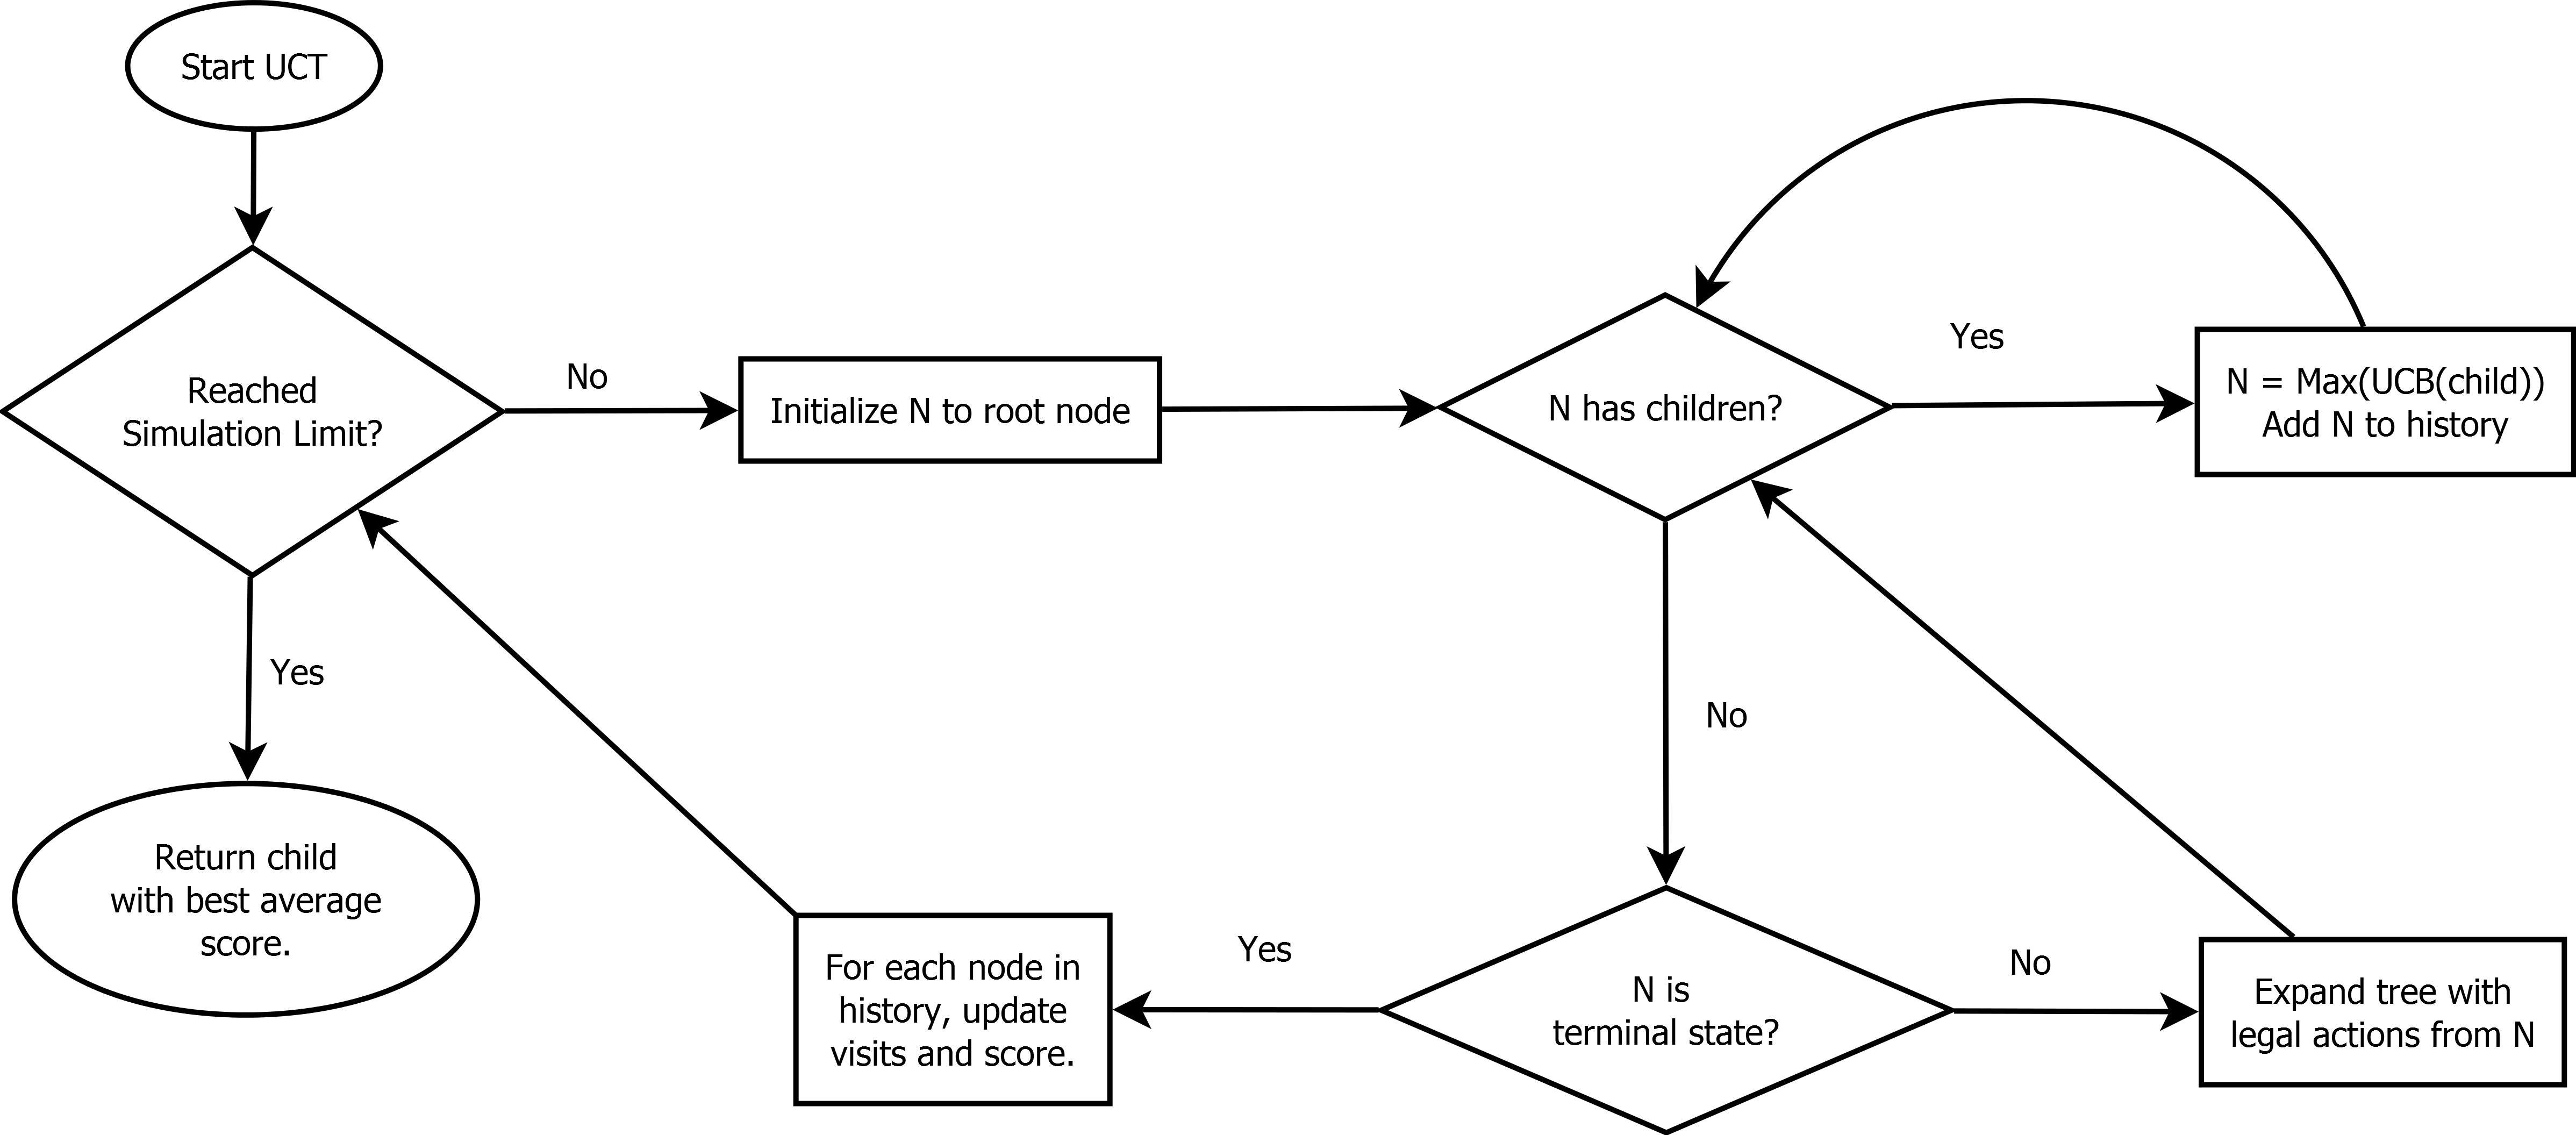
\includegraphics[width=\linewidth]{uct.png}
\caption{The basic UCT algorithm for searching over an MDP. Equation \ref{eqn:uct} is
the UCB algorithm referenced in the child selection step.}
\label{uct-diagram}
\end{figure}

A recently popular PP algorithm is the Upper Confidence bound applied to Trees (UCT)\cite{kocsis_bandit_2006}.
This algorithm is detailed in Figure \ref{uct-diagram}.
Online planning in MDPs generally follows two steps. From each state
encountered, a lookahead tree is constructed and used to estimate the
utility of each action in this state. Then, the best action is taken,
the system transitions to the next state and the procedure is
repeated. In order to build a lookahead tree, a ``rollout policy'' is
used. This policy has two components: if it encounters a state already
in the tree, it follows a ``tree policy,'' discussed further below. If
it encounters a new state, the policy reverts to a ``default'' policy
that typically randomly samples an action. In all cases, any rewards
received during the rollout search are backed up. Because this is a
Monte Carlo estimate, typically, several simultaneous trials are run,
and we keep track of the rewards received by each choice and
use this to select the best action at the root.

The final detail that UCT specifies is the method for determining the tree policy.
The tree policy needed by UCT for a state $s$ is the action $a$ in that state which maximizes:
\begin{equation}
P(s,a) = Q(s,a) + c\sqrt{\frac{ln N(s)}{N(s,a)}}\label{eqn:uct}
\end{equation}
Here $Q(s,a)$ is the estimated value of $a$ as observed in the tree
search and $N(s)$ and $N(s,a)$ are visit counts for the state and
state-action pair. Thus the second term is an exploration term that
biases the algorithm towards visiting actions that have not been
explored enough. $c$ is a constant that trades off exploration and
exploitation. This essentially treats each action decision
as a ``bandit problem" where the best action is determined by iteratively
exploring the branches of the action tree that previous experiments
have shown to be best.  Previous work \cite{uct-go} shows that this approach can
efficiently select near-optimal actions at each state.


\section{Probabilistic Lexicalized Tree Adjoining Grammars}

A grammar is a set of rules which define strings that are contained within a language.
Many artificial languages, especially programming languages like C or Java, have
grammars which can be expressed concisely and without ambiguity.  Some
constructed languages, like Lojban \cite{lojban}, also have this property.

Natural languages (e.g. English), however, are well-known to have grammars which are difficult
to represent with any single given formalism \cite{klein2012context}. There are many possible
formalisms which can contain the rules that make up
a grammar.  Most of these formalisms involve a form of "rewriting", which
is to say, replacing a nonterminal token in a string with a specific set of
terminals and nonterminals.

A Tree Adjoining Grammar (TAG) takes a different approach, differing substantially from the more
common CFGs and PCFGs.
TAGs are tree-based grammars consisting of two sets of trees, called initial
trees and adjoining trees (sometimes ``auxiliary trees").  These two kinds of trees tend to perform
different roles semantically in addition to their differing syntactic roles.  The former,
initial trees, are usually for adding new semantic information to the sentence.  They
add new nodes to the sentence tree.  In a simplified TAG of English,
initial trees contain rules like ``Verb Phrases contain a Verb and a Noun", or ``VP $\rightarrow$ V N".
A sentence can be made entirely of initial trees, and must contain at least
one initial tree.  An example of an initial tree is shown in Figure \ref{initial-tree-example}.

\begin{figure}[ht]
\centering
\begin{minipage}[b]{0.45\linewidth}
\centering
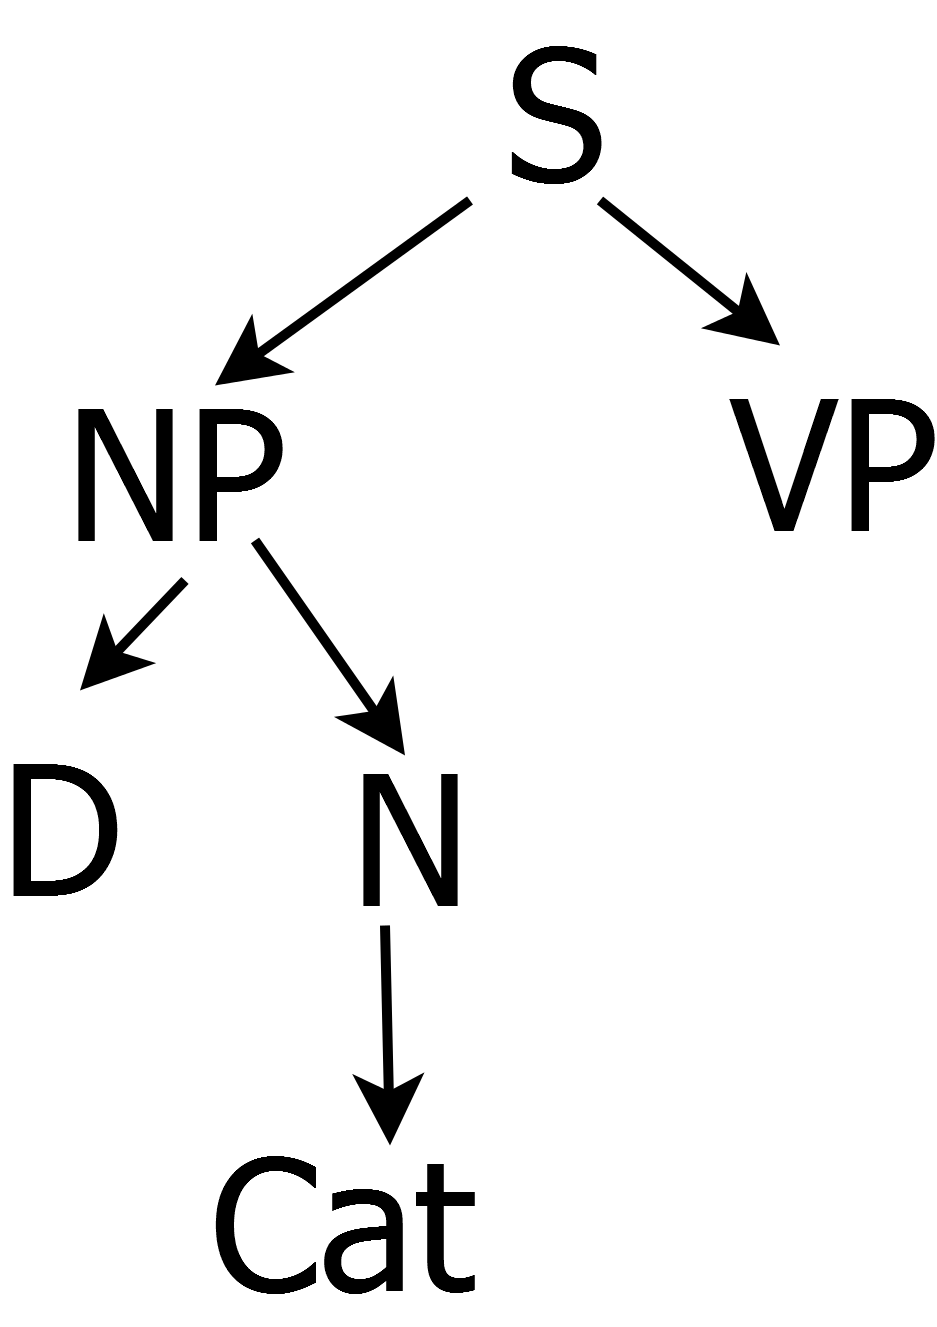
\includegraphics[width=0.5\linewidth]{initial-example.png}
\caption{An example of an initial tree in a lexicalized tree adjoining grammar}
\label{initial-tree-example}
\end{minipage}
\quad
\begin{minipage}[b]{0.45\linewidth}
\centering
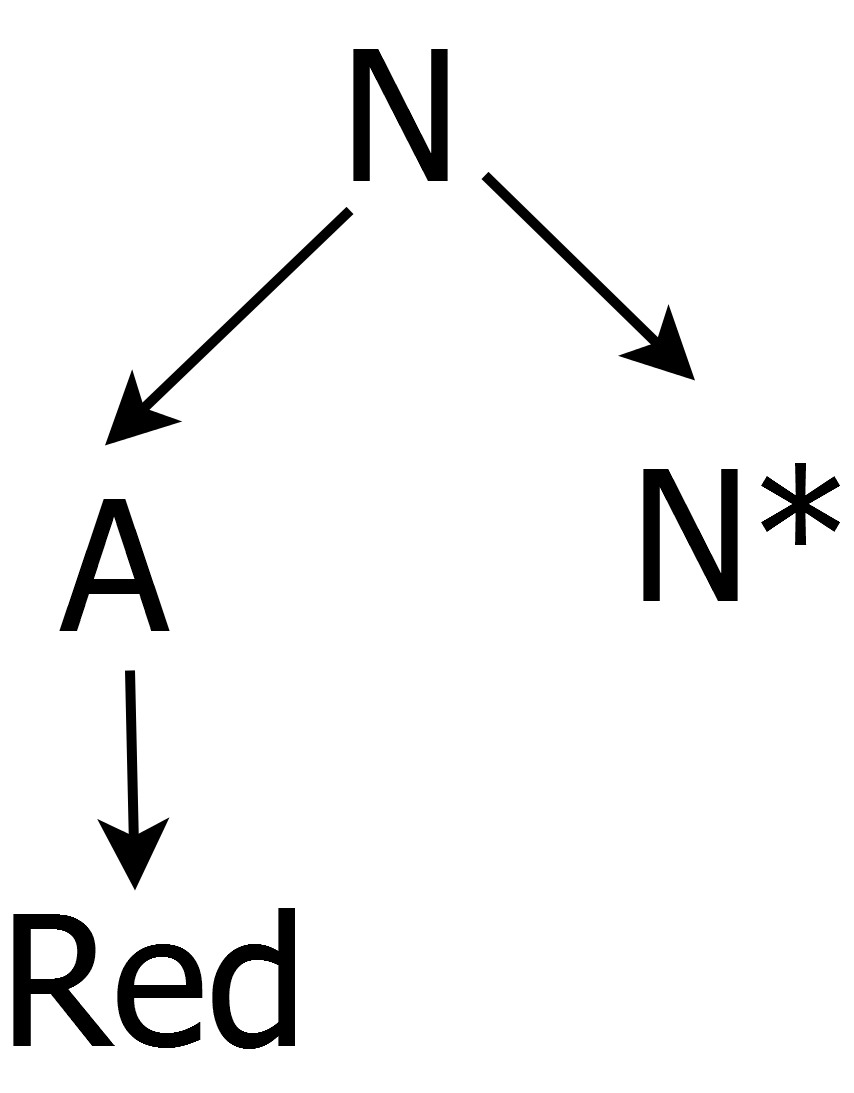
\includegraphics[width=0.5\linewidth]{adjoining-tree-example.png}
\caption{An example of an adjoining tree in a lexicalized tree adjoining grammar}
\label{adjoining-tree-example}
\end{minipage}
\end{figure}

This tree has as its root the S node, and this defines how it can interact with other
trees under a TAG.  Since this is an initial tree, it can only interact with other trees by
substitution.  That is, this tree is a drop-in replacement for an S node with no children.
This is how we get from our stub sentence (S) to a complete sentence.

Adjoining trees usually clarify a point in a sentence.  In a simplified TAG of English, adjoining
trees would contain rules like ``a noun can have an adjective placed in front of it," or ``N $\rightarrow$ A N".
An example of an adjoining tree is shown in Figure \ref{adjoining-tree-example}.

This tree has as its root an N node.  It also has a specially annotated N node elsewhere in the
tree.  These nodes define its interaction with other trees under a TAG.  Adjoining trees interact
with other trees only by ``adjoining".  In an adjoining action, we select the node
to adjoin to, which must be of the same label as the root node of the adjoining tree.  We remove
that node from the other tree and put the adjoining tree in its place.  Then
we place that original node into the adjoining tree as a substitution for the foot node.
For example, if we had the tree in Figure \ref{tree-1} and we wanted to adjoin the example adjoining tree
in Figure \ref{adjoining-tree-example}, we would first create the intermediate tree in Figure \ref{tree-2},
and then perform the substitution and get the tree in Figure \ref{tree-3}.  Notice that this has the effect,
in all cases, of making the tree deeper.

\begin{figure}[ht]
\centering
\begin{minipage}[b]{0.3\linewidth}
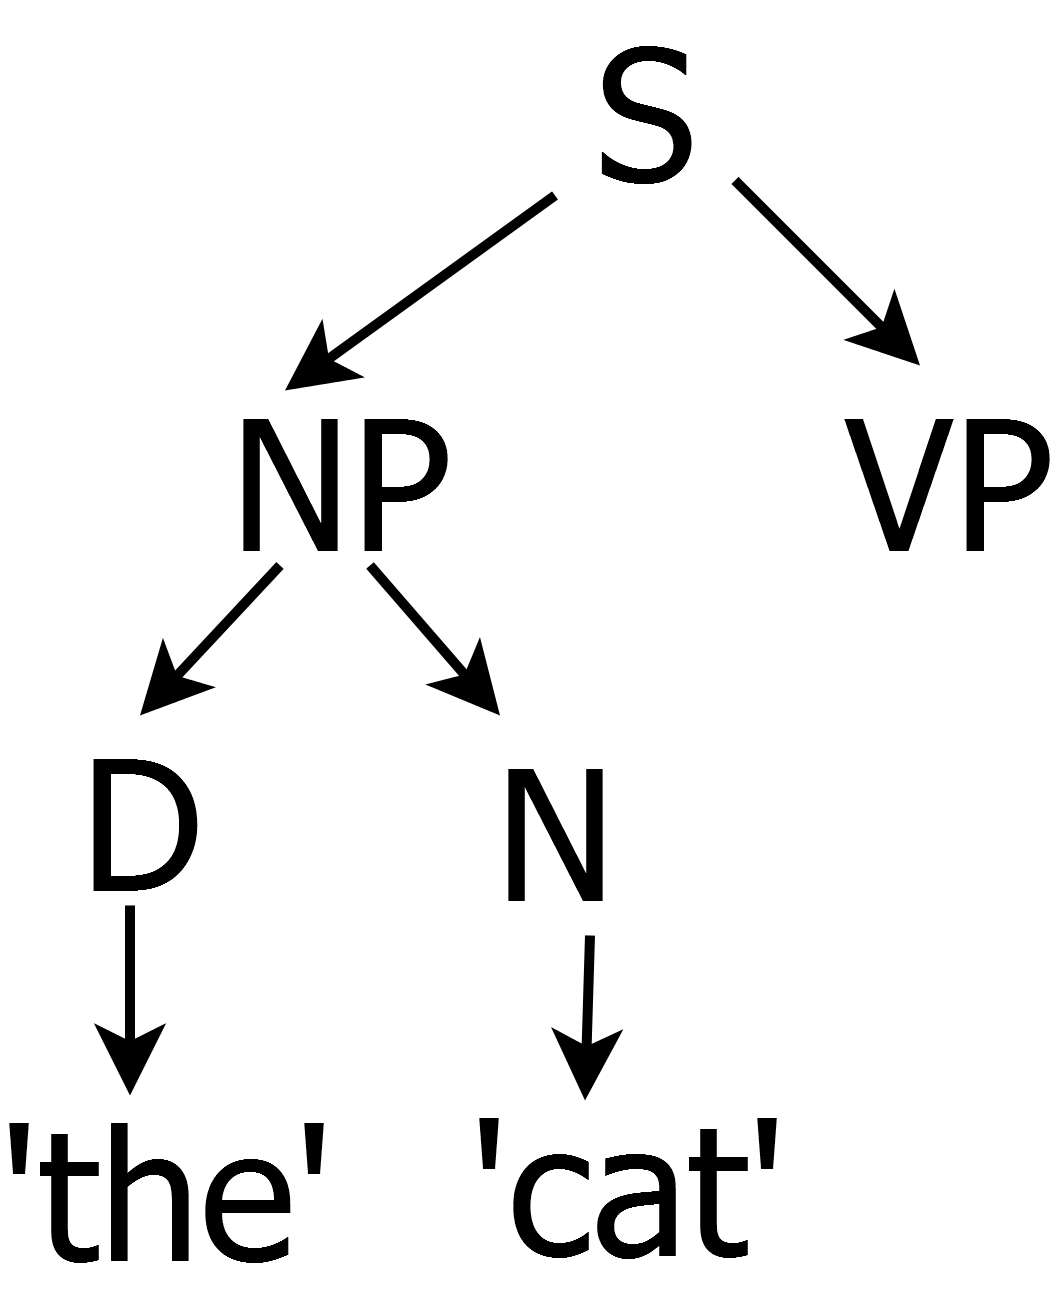
\includegraphics[width=\linewidth]{tree-1.png}
\caption{Partial tree}
\label{tree-1}
\end{minipage}
\quad
\begin{minipage}[b]{0.3\linewidth}
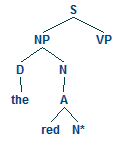
\includegraphics[width=\linewidth]{tree-2.png}
\caption{Intermediate tree}
\label{tree-2}
\end{minipage}
\quad
\begin{minipage}[b]{0.3\linewidth}
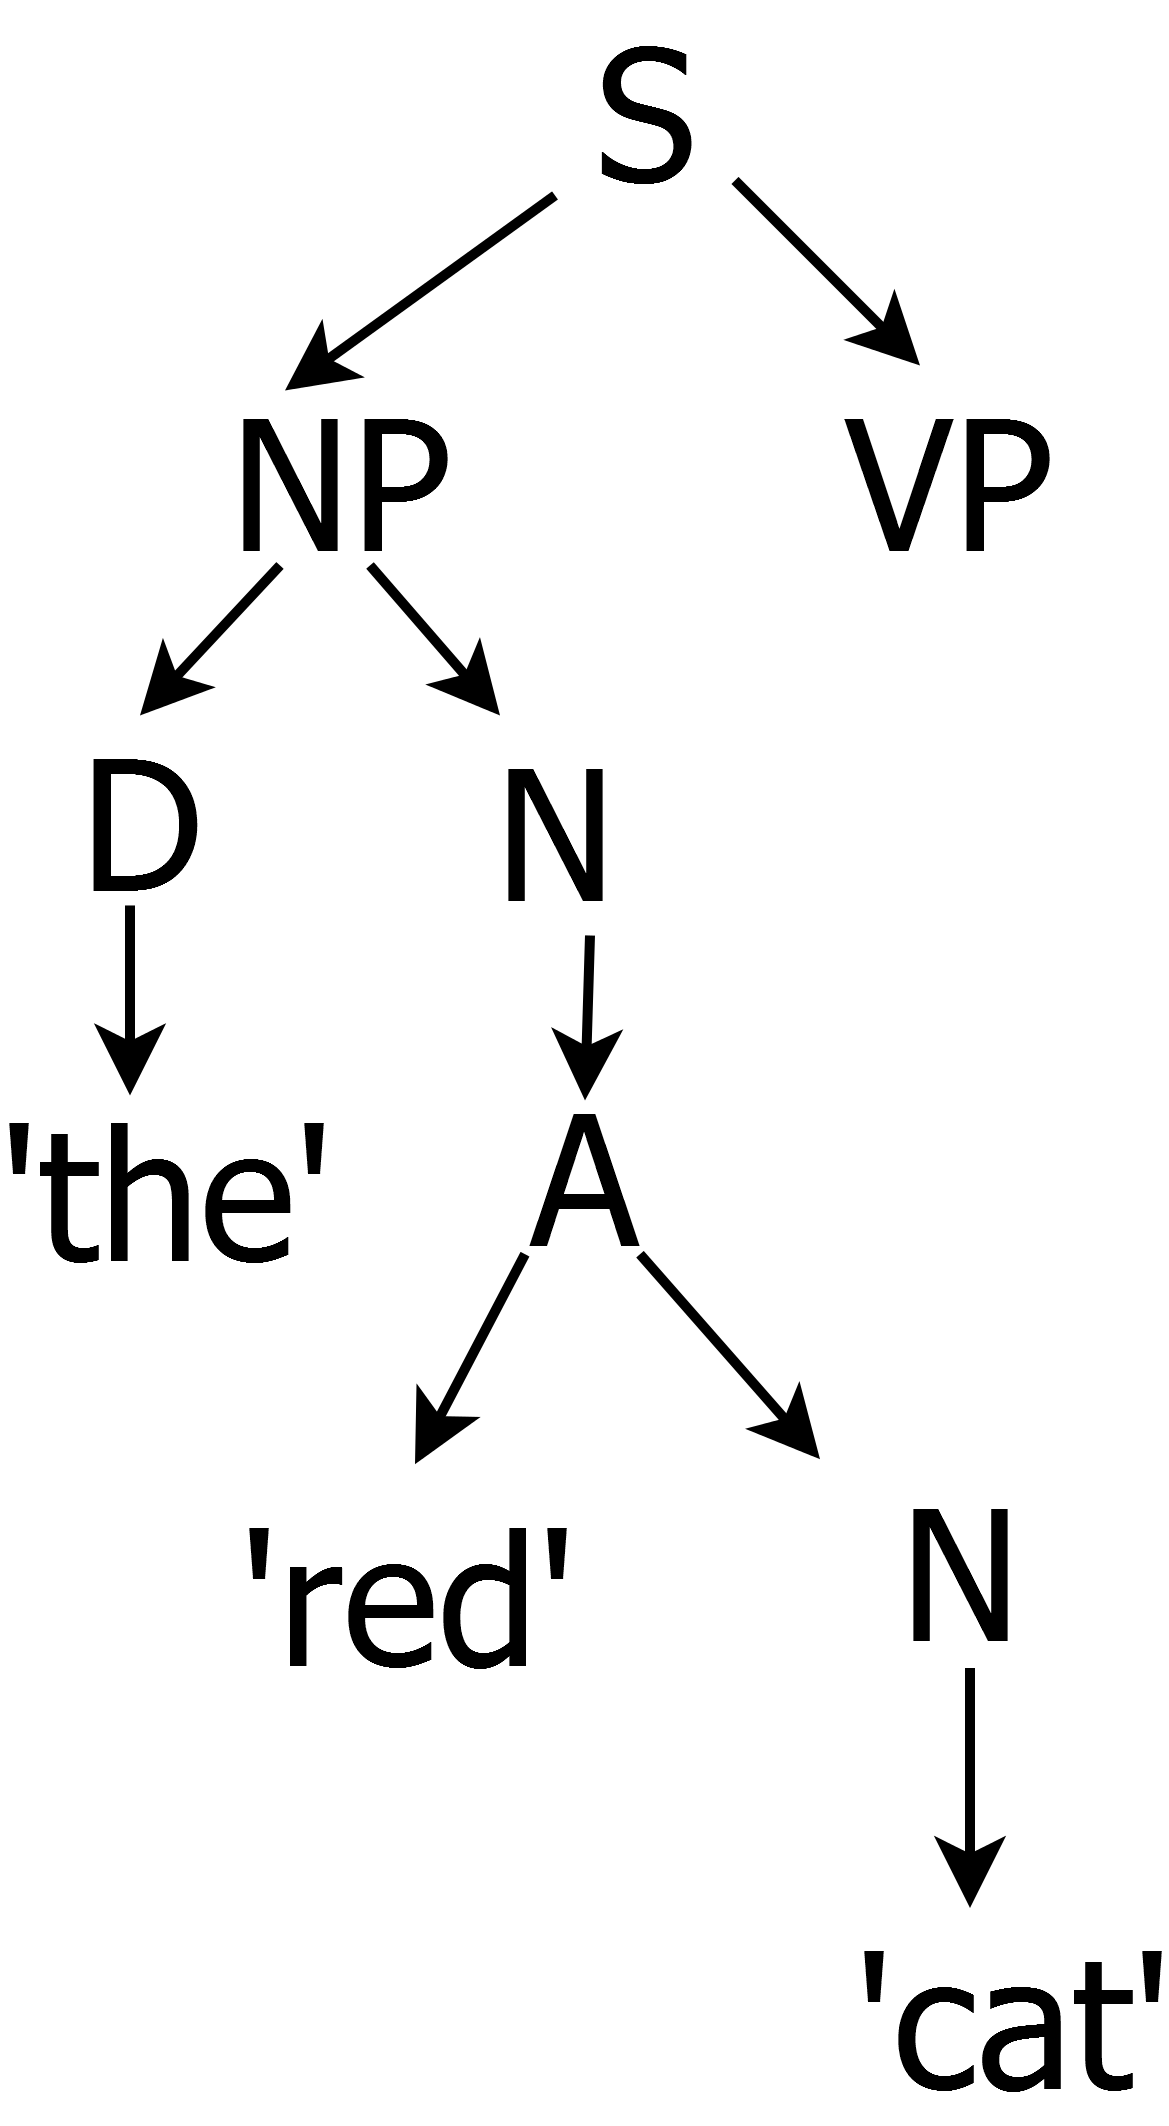
\includegraphics[width=\linewidth]{tree-3.png}
\caption{Final tree}
\label{tree-3}
\end{minipage}
\end{figure}

We use a variation of TAGs in our work, called a probabilistic lexicalized TAG (PLTAG), where each tree is
associated with a lexical item called an anchor.  All examples given above are examples of
lexicalized trees.  An example of an unlexicalized tree would be (NP (D) (N)), where there
are no nodes containing lexical tokens.  The probabilistic component comes into these trees
as a way to represent the fact that not all trees are equal.  Some trees are more common
than others, and PLTAGs represent that fact with probabilities assigned to each tree.
The probabilities of each class of trees (substitution / adjoining) with the same root node
will sum to 1, in order to ensure that there is a well-defined probability distribution
over the choices for substitution or adjoining at a single node in a tree.

The XTAG project has had some success using LTAGs to model English grammar\cite{xtag}, 
so we focus mostly on LTAGs in our work.
\chapter{Related Work}
\section{Approaches to NLG}
Two broad categories of
approaches have been used to attack the general NLG problem. One
direction can be thought of as ``overgeneration and ranking.'' Here
some (possibly probabilistic) structure is used to generate multiple
candidate sentences, which are then ranked according to how well they
satisfy the generation criteria. This includes work based on chart
generation and
parsing~\cite{shieber_uniform_1988,kay_chart_1996}. These generators
assign semantic meaning to each individual token, then use a set of
rules to decide if two words can be combined.  Any combination which
contains a semantic representation equivalent to the desired meaning 
is a valid output from a chart generation
system. Another example of this idea is the HALogen/Nitrogen
family of systems~\cite{langkilde_2002_halogen}. HALogen uses a two-phase
architecture where first, a ``forest'' data structure that compactly
summarizes possible expressions is constructed.  The structure allows
for a more efficient and compact representation compared to lattice
structures that had been previously used in statistical sentence
generation approaches.  Using dynamic programming, the highest ranked
sentence from this structure is then output. Many other systems using
similar ideas exist, e.g.~\cite{white_2003_ccg,lu2009natural}.

A second line of attack formalizes NLG as an AI planning problem.
SPUD \cite{stone_2003_spud}, a system for NLG through microplanning,
considers NLG as a problem which requires realizing a deliberative
process of goal-directed activity.  Many such NLG-as-planning systems
use a pipeline architecture, working from their communicative goal
through a series of processing steps and concluding by outputting the
final sentence in the desired natural language. This is usually done
into two parts:
discourse planning and sentence generation. In
discourse planning, information to be conveyed is selected and split
into sentence-sized chunks. These sentence-sized chunks are then sent
to a {\em sentence generator}, which itself is usually split into two
tasks, {\em sentence planning} and {\em surface realization}
\cite{koller_experiences_2011}.  The sentence planner takes in a
sentence-sized chunk of information to be conveyed and enriches it in
some way.  This is then used by a {\em surface realization}
module which encodes the enriched semantic representation into 
 natural language.  This chain is sometimes referred to as the
``NLG Pipeline'' \cite{reiter_building_2000}.  Our approach is
part of this broad category.

Another approach, called {\em integrated generation}, considers both
sentence generation portions of the pipeline together.
\cite{koller_sentence_2007}.  This is the approach taken in some
modern generators like CRISP \cite{koller_sentence_2007} and PCRISP
\cite{bauer_sentence_2010}.  In these generators, the input semantic
requirements and grammar are encoded in PDDL~\cite{fox2003pddl2},
which an off-the-shelf planner such as
Graphplan~\cite{blum_1997_graphplan} uses to produce a list of
applications of rules in the grammar.  These generators generate
parses for the sentence at the same time as the sentence, which keeps
them from generating realizations that are grammatically incorrect,
and keeps them from generating grammatical structures that cannot be
realized properly. PCRISP extends CRISP by adding support for
probabilistic grammars. However the planner in PCRISP's back end is
still a standard PDDL planner, so PCRISP transforms the probabilities
into costs so that a low likelihood transition has a high cost in
terms of the plan metric.

\section{Grammar Representation}

In the NLG-as-planning framework, the choice of grammar representation
is crucial in treating NLG as a planning problem; the grammar provides
the actions that the planner will use to generate a sentence.  Tree
Adjoining Grammars (TAGs) are a common choice
\cite{koller_sentence_2007} \cite{bauer_sentence_2010}. TAGs are
tree-based grammars consisting of two sets of trees, called initial
trees and auxiliary or adjoining trees.  An entire initial tree can
replace a leaf node in the sentence tree whose label matches the label
of the root of the initial tree in a process called ``substitution.''
Auxiliary trees, on the other hand, encode recursive structures of
language.  Auxiliary trees have, at a minimum, a root node and a foot
node whose labels match.  The foot node must be a leaf of the
auxiliary tree.  These trees are used in a three-step process called
``adjoining''.  The first step finds an adjoining location by
searching through our sentence to find any subtree with a root whose
label matches the root node of the auxiliary tree.  In the second
step, the target subtree is removed from the sentence tree, and placed
in the auxiliary tree as a direct replacement for the foot node.
Finally, the modified auxiliary tree is placed back in the sentence
tree in the original target location. We use a variation of TAGs in
our work, called a lexicalized TAG (LTAG), where each tree is
associated with a lexical item called an anchor.

Though the NLG-as-planning approaches are elegant and appealing, a key
drawback is the difficulty of handling probabilistic grammars, which
are readily handled by the overgeneration and ranking
strategies. Recent approaches such as
PCRISP~\cite{bauer_sentence_2010} attempt to remedy this, but do so in
a somewhat ad-hoc way, because they rely on deterministic planning to
actually realize the output. In this work, we directly confront this
by switching to a more expressive underlying formalism, a Markov
decision process (MDP). We show in our experiments that this
modification has other benefits as well, such as being anytime and an
ability to handle complex communicative goals beyond those that
state-of-the-art deterministic planners can currently solve.

We note that though the application of MDPs to NLG appear not to have
been explored, some preliminary work has explored the application of
MDPs and the UCT algorithm~\cite{chevelu_introduction_2009} that we
also use in our work to paraphrasing. Here the algorithm was used to
search through a paraphrase table to find the best paraphrase solution.

\section{NLG Applications}

The work we describe here addresses the pure NLG problem without
considering the surrounding context; in practice, such a system would
be integrated into a larger system, such as one carrying out a
dialog. However, we note that many dialog systems, such as
NJFun~\cite{litman_njfun_2000}, model dialog using reinforcement
learning. While integrating our NLG approach with such a system is a
direction for future work, the similarity of the formalism indicates
it should be feasible.
NLG has many applications, but one which is of particular interest is
natural language interfaces, or dialog systems.  Recently, such
systems have generated a good deal of interest in mobile devices,
though their origin goes back to GUS and similar systems developed at PARC
in the 1970s \cite{bobrow_gus_1977}.  These systems take input from a user
in the form of natural-language speech or text, process that information in 
some way (i.e. running a query against a knowledge base as NJFun does
\cite{litman_njfun_2000}), then return a response to the user in
natural English.  This interaction proceeds by turns in much the same way
as a natural dialog between humans.  The dialog system is responsible
for managing the state of the dialog.  By the point that an output realizer is 
needed, the discourse planning step of the NLG pipeline has already been
completed.
\chapter{Natural Language Generation As Probabilistic Planning}
\section{NLG as planning in an MDP}
We formulate NLG as a planning problem on a Markov decision process
(MDP)  Using such an approach with a suitable defined MDP
(explained below) allows us to naturally handle
probabilistic grammars as well as formulate NLG as a planning problem,
unifying the distinct lines of attack described above. Further, the
strong theoretical guarantees of UCT translate into fast generation in
many cases, as we demonstrate in our experiments.
As the state space size in the language generation MDP is
very large, we use a variation of the UCT algorithm in our system,
described below.

\section{The UCT Algorithm}

Online planning in MDPs generally follows two steps. From each state
encountered, a lookahead tree is constructed and used to estimate the
utility of each action in this state. Then, the best action is taken,
the system transitions to the next state and the procedure is
repeated. In order to build a lookahead tree, a ``rollout policy'' is
used. This policy has two components: if it encounters a state already
in the tree, it follows a ``tree policy,'' discussed further below. If
it encounters a new state, the policy reverts to a ``default'' policy
that typically randomly samples an action. In all cases, any rewards
received during the rollout search are backed up. Because this is a
Monte Carlo estimate, typically, several simultaneous trials are run,
and we keep track of the rewards received by each choice and
use this to select the best action at the root.

The final detail that UCT specifies is the method for determining the tree policy.
The tree policy needed by UCT for a state $s$ is the action $a$ in that state which maximizes:
\begin{equation}
P(s,a) = Q(s,a) + c\sqrt{\frac{ln N(s)}{N(s,a)}}\label{eqn:uct}
\end{equation}
Here $Q(s,a)$ is the estimated value of $a$ as observed in the tree
search and $N(s)$ and $N(s,a)$ are visit counts for the state and
state-action pair. Thus the second term is an exploration term that
biases the algorithm towards visiting actions that have not been
explored enough. $c$ is a constant that trades off exploration and
exploitation. This essentially treats each action decision
as a bandit problem; previous work shows that this approach can
efficiently select near-optimal actions at each state.

\section{STRUCT}
\subsection{Overview}
We now describe our approach, called Sentence Tree Realization with
UCT (STRUCT). The states of the underlying MDP contain {\em partial
 sentences} along with their parse trees and semantic annotations.
The actions available at a
state allow refinements to the partial sentences. In particular, the
algorithm may choose an available nonterminal in the current parse
tree for a substitution, or choose any nonterminal for an adjoin operation from a (possibly
probabilistic) LTAG. Given a nonterminal choice and a fixed
probabilistic lexicalized TAG (PLTAG), a well defined probability
distribution is induced over possible next states (possibly uniform if
just an LTAG is used).   Since trees in LTAGs are associated
with individual words, they can be interpreted as adding a specific
semantic meaning to the overall sentence while describing precisely
the syntactic environment in which these words can occur, and can even
define any arguments for the word in question, for instance, the
location of the subject and object of a verb, or the presence of a
required third argument.  Further, since all recursive phenomena are
encoded in auxiliary trees, it factors recursion from the domain of
dependencies \cite{bauer2009statistical}, and can add auxiliary trees
to partial sentences without breaking dependency links between nodes.
In situations where the sentence is complete (no nonterminals without
children), we add a dummy action to stop generation and emit the
sentence.  Note that a complete sentence does not necessarily imply
a terminal state because adjoin operations can still be performed
(e.g. ``The dog ran'' could be expanded to ``The black dog ran quickly'').

In order to control the search space, we restrict the structure of the
MDP so that while substitutions are available, only those operations
are considered when determining the distribution over the next state,
without any adjoins.  We do this is in order to generate a
complete and valid sentence quickly.  This allows STRUCT to operate as
an anytime algorithm, described further below.

 The transition distribution in
 the underlying MDP is implicitly defined by the probabilities
 associated with a PLTAG, or uniform in the case of a standard LTAG.
\begin{figure}[t]
\centering
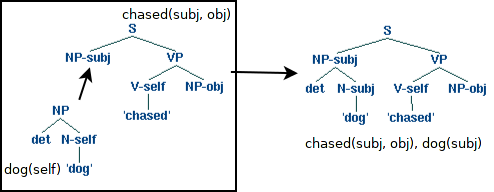
\includegraphics[width= 0.7 \linewidth]{sub-example.png}\label{examples-s}
\caption{An example tree substitution operation in STRUCT.}
\end{figure}

\begin{figure}[t]
\centering
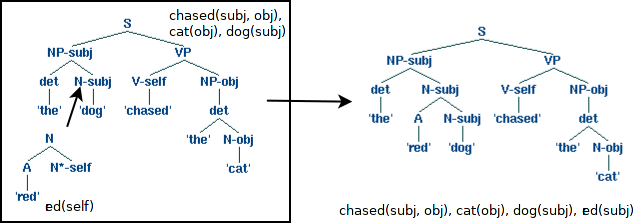
\includegraphics[width= 0.7 \linewidth]{adjoin-example.png}\label{examples-a}
\caption{An example tree adjoining operation in STRUCT.}
\end{figure}

\subsection{Grammar Description}
 In order to interact with the communicative goal, each word in our
 grammars consists of two components, a grammar entry and a lexicon
 entry.  A grammar entry has a name, a tree, and a set of annotations.
 These annotations contain data about how the syntactic data (the tree
 itself) interacts with the semantic data.  A lexicon entry has a word
 and a list of meanings.  These meanings are written as functions in
 first order logic, and can use as arguments the objects defined by
 the tree. This representation is similar to that used by
 CRISP~\cite{koller_sentence_2007}. In Figure~\ref{examples-s}
  we show an example of a substitution operation applying an LTAG production to
 a chosen nonterminal in a partial sentence, and the associated
 semantic information.  Figure \ref{example-a} similarly shows an example
 of an adjoining operation.

\section{Specifications of Inputs}

\subsection{Grammar Specification}

A grammar, for our purposes, contains a set of trees, divided into two sets (initial and auxiliary).
These trees need to be annotated with the entities in them.  Entities are defined as any element
anchored by precisely one node in the tree which can appear in a proposition representing the
semantic content of the tree.  These trees are uniquely named, and also contain an
annotation (+) representing the lexicalized node.  See Appendix A for an example of a combined
grammar / lexicon.

\subsection{Lexicon Specification}

The lexicon that we use is a list of permissible word-tree pairings, annotated with the meaning of
the pairing.  For instance, if the grammar contained a tree named "a.adj", (N (A+) (N-foot*))
(an adjoining tree for prepending an adjective to a noun, whose foot node is an entity named "foot"),
then the lexicon might contain an entry "a.adj: ['red', 'red(foot)]".  That would mean that the overall
LTAG that we are using contains the tree named "a.adj", lexicalized to 'red', and that when that tree
is applied to a sentence, the sentence's meaning is adjusted to include red(name of the foot node).
Appendix A contains an example of a combined grammar / lexicon.

\subsection{Communicative Goal Specification}

The communicative goal is just a list of propositions with dummy entity names.  Matching entity
names refer to the same entity; for instance, a communicative goal of 'red(d), dog(d)' would
match a sentence with the semantic representation 'red(subj), dog(subj), cat(obj), chased(subj, obj)',
like "The red dog chased the cat", for instance.  As shown here, the communicative goal does
not have to refer to any "central meaning" of the sentence as a human would select it, but rather
to propositions which the sentence affirms.  Appendix B contains an example of a communicative
goal and a number of sentences which satisfy it.

\subsection{Reward Function}
 While the production probabilities in the given PLTAG define the
 global structure of the state space, we use the reward function of
 the MDP to encode the specific communicative goal we are after. Since
 each state contains a partial sentence with its associated semantic
 information, we use this to evaluate the algorithm's progress towards
 the goal, and reward is allocated based on this progress. A key
 advantage of STRUCT over current techniques is our ability to specify
 a detailed reward function that captures complex communicative goals.
 For example, we can give ``progress'' rewards for partial sentences
 that achieve some parts of the communicative goal; we can penalize
 the algorithm if it attempts to generate a sentence that communicates
 something we wish {\em not} to communicate; we can trade off the
 importance of multiple communicative goals in the same sentence; we
 can even set up the reward function to prefer global criteria such as
 ``readability'', if we so choose. Of course, once any sentence is
 found that achieves the complete communicative goal, a large reward
 is given. Since the algorithm keeps track of the cumulative reward,
 such a sentence becomes a candidate solution. During the search,
 since we use finite depth lookahead and wish to propagate long range
 rewards to the root, we use a discount factor of 1.

\subsection{Execution as an Anytime Algorithm}
 With the MDP definition above, we use UCT to find a solution sentence
 (Algorithm~\ref{uct-code}). We modify the standard algorithm in two
 ways. First, in the action selection step, we select the action that
 leads to the best $P(s,a)$ over all simulations rather than the best
 {\em average} $P(s,a)$. We do this because the original formulation
 of UCT is designed to work in adversarial situations, in such cases,
 selecting the absolute best may be risky if the opponent can respond
 with something that can also lead to a very bad result. In our case,
 however, there is no opponent, so we can freely choose the action
 leading to best overall reward. Second, after every action is
 selected and applied, we check to see if we are in a state in which
 the algorithm could terminate (i.e. the sentence has no nonterminals
 yet to be expanded).  If so, we determine if this is the best
 possibly-terminal state we have seen so far.  If so, we store it, and
 continue the generation process. If we reach a state from which we
 cannot continue generating, we begin again from the start state of
 the MDP. Because of the structure restriction above (substitution
 before adjoin), STRUCT also generates a valid sentence quickly. These
 modifications enable STRUCT to perform as an anytime algorithm, which
 if interrupted will return the highest-value complete and valid
 sentence.

After this point, any time that there are no substitutions
available (all nonterminals have at least one child), we record the
current sentence and its associated reward.  Such a sentence is
guaranteed to be both grammatical and complete.  If generation is
interrupted, we return the highest-value complete and valid sentence.
In this way, our approach functions as an anytime algorithm.

 We note that neither of these modifications cause any loss of
 generality.  Our Anytime-UCT implementation will work on any suitably
 defined MDP.  We implemented the system in Python 2.7. The pseudocode
  is shown in Algorithm~\ref{uct-code}.

 Clearly, the action set can get very large for a large grammar or for
 a long sentence with many locations for adjoining.  Still, this is the
 only way to ensure that we can generate all possible grammatical
 sentences.  UCT deals very well with this large action set due to the
 pruning inherent in its iterated Monte Carlo sampling method.  We can
 further compensate for this large action set by increasing the number
 of samples, if necessary.  It should also be noted that most
 combinations of these actions are order-independent; for instance, two
 actions, each adjoining an adjective to the subject and object of the
 sentence, respectively.  It is also notable that, occasionally, the
 order of some words in a sentence is not important.  ``A small white
 teapot'' and ``a white small teapot'' convey the same semantic
 information despite the different ordering of their adjectives.

\subsection{Algorithm Details}
\begin{figure}
\caption{The STRUCT Algorithm.}\label{uct-code}
\begin{algorithmic}[1]
\REQUIRE Number of simulations $numTrials$, Depth of lookahead $maxDepth$
\ENSURE Generated sentence tree
\STATE $bestSentence \gets$ nil
\WHILE {User has not interrupted generation}
\STATE $state \gets$ empty sentence tree
\WHILE{$state$ not terminal}
	\FOR{$numTrials$}
		\STATE $testState \gets state$
		\STATE $currentDepth \gets 0$
		\IF{$testState$ has unexplored actions}
			\STATE Apply one unexplored PLTAG production chosen
                        uniformly at random to $testState$
			\STATE $currentDepth$++
		\ENDIF
		\WHILE{$currentDepth < maxDepth$}
			\STATE Apply PLTAG production selected by tree
                        policy (Equation~\ref{eqn:uct})
			\STATE $currentDepth$++
		\ENDWHILE
		\STATE calculate reward for $testState$
		\STATE associate reward with first action taken
	\ENDFOR
	\STATE $state \gets$ maximum reward $testState$
	\IF{$state$ score $> bestSentence$ score \AND $state$ has no nonterminal leaf nodes}
		\STATE $bestSentence \gets state$
	\ENDIF
\ENDWHILE
\ENDWHILE
\RETURN $bestSentence$
\end{algorithmic}
\end{figure}

UCT(Upper Confidence bound applied to Trees) \cite{kocsis_bandit_2006} is a planning algorithm that takes advantage of
Monte-Carlo sampling to prune large sections of the search space each iteration. Actions are sampled from each possible
action at each state, and an action is chosen immediately based on the best average reward found. This algorithm can
handle large search-spaces since it prunes a large percentage of the search space with each action. As it takes more
samples per round, it increases the likelihood that it will prune only portions of the search space that do not contain
the best output increases.\\

Our modifications of UCT in order to improve its use in the specific natural language generation task are show in Figure
\ref{uct-code}. Unlike in the game-playing task for which UCT was designed, we have no adversary in this generation
task, and therefore we seek the best path that we have found so far, rather than the maximum average-value path. We have
found that UCT, modified in this way, provides excellent optimal and near-optimal outputs. In addition, due to the way
that we have structured our action definition, we use UCT as an anytime algorithm; we first generate the simplest and
shortest valid sentence first, and increasingly improve the sentence over time until the sentence can no longer be
improved.\\

Our choice of UCT is motivated by the high branching factor encountered in natural language generation when dealing with
large grammars as well as the belief that optimal sentences to accomplish a communicative goal are not required in most
discourse. In fact, generating optimal sentences may be more time-consuming than nearly-optimal plans which accomplish
the goal nearly as well.\\

The process of generation can be split into four components:
\begin{enumerate}
\item Tree Policy
\item State Expansion
\item Default Policy
\item Reward Assignment
\end{enumerate}

\subsubsection{Tree Policy}
Starting from the current state, an action will repeatedly be chosen based on a balance of exploration and exploitation,
until a state with an open action is hit, a leaf is hit, of the depth limit is reached. The balance between exploration
and exploitation is maintained by probabilistically selecting actions based on their expected value and the number of
samples taken from that state. More precisely:

$$P(a) = Q(s,a) + c\sqrt{\frac{ln n(s)}{n(s,a)}}$$

where $a$ is an action, $s$ is the current state, $c$ is the algorithm's exploration constant, $n(s)$ is the number of
times state $s$ has been encountered, $n(s,a)$ is the number of times action $a$ was taken in state s, and $Q(s,a)$ is
the expected value of state $s$ after selecting action $a$.

\subsubsection{State Expansion}
If there are any unexplored actions for the current state, choose one of the unexplored actions according to an
arbitrary heuristic. Heuristic choice is described below.

\subsubsection{Default Policy}
Continue to select actions at random until either a terminal state or the depth limit is reached.

\subsubsection{Reward Assignment}
Calculate the reward function for the state that results after executing all of the chosen action and push the reward
all the way back up to the root node representing the current state.

\subsection{Grammar Choice}

STRUCT supports Context Free Grammars (CFGs), Probabilistic Context Free Grammars (PCFGs), Tree Adjoining Grammars
(TAGs), and Probabilistic Tree Adjoining Grammars (PTAGs). For the experiments below, we primarily focus on a restricted
subset of TAGs and PTAGs, the Lexicalized Tree Adjoining Grammars (LTAGs, PLTAGs). LTAGs are TAGs in which each tree
contains at least one word which will be present in the final sentence, an 'anchor word'. CRISP, mentioned above, also
uses LTAGs, which makes comparison between the generators simpler.\\

LTAGs were chosen due to their interesting linguistic properties. Since trees are associated with individual words, they
can be interpreted as adding a specific semantic meaning to the overall sentence while describing precisely the
syntactic environment in which these words can occur, and can even define any arguments for the word in question, for
instance, the location of the subject and object of a verb, or the presence of a required third argument. Further, since
all recursive phenomena are encoded in auxiliary trees, we have removed recursion from the domain of dependencies
\cite{bauer2009statistical}, and can add auxiliary trees to our partial sentences without breaking dependency links
between nodes.

\subsection{Action Definition}

Actions in STRUCT are applications of a particular grammar rule to a specific node in the partial tree. In a
context-free grammar and in the case of an initial tree in a TAG, these are determined by iterating through all leaf
nonterminals and adding a possible action for each rule in the grammar applicable at this point. Adjoining trees in a
TAG are determined by iterating through each node in the tree and adding a possible action for each adjoining tree
applicable at that point.\\

 \subsection{Reward Function Definition}

 The reward function for a state must be defined exclusively in terms
 of the state in question.  The reward function serves as a metric to
 rank the favorableness of a sentence.  This reward function must be
 efficiently computable since it will be computed for every iteration
 in the UCT algorithm.  It must also be able to provide a value for a
 partial sentence since, due to the depth limit, a complete sentence
 may not always be reached.\\
 
 We found that there are several possible reward functions which will
 return satisfactory results on a variety of experiments.  The reward function
 which we found to be nearly universally useful considers a goal as well as a 
 grounded world.  It examines all possible mappings of entities present in
 a given sentence's annotation to entities present in the world, then returns
 a high value if there are any mappings which are both possible (contain no statements
 which are not present in the grounded world) and fulfill the goal (contain the
 goal statement).\\

This reward function happens to perform somewhat slowly since it includes
a subsumption problem as a step within it.  It performs in $O(N!)$ time, where
N is the number of entities present in the sentence.  We refer to this algorithm as
"perfect evaluation".\\

Since on occasion we will not need the power of a perfectly correct algorithm,
it's worthwhile to consider alternate algorithms.  One such algorithm assumes that
the given sentence is correct and that all entity references are appropriate, then
searches for statements in the sentence which contradict this assumption.  This
algorithm obviously runs much faster but has limitations.  One such limitation is
that such an approach cannot perform an explicit mapping of entities in the sentence
to entities in the world, which means that some sentences which do not precisely
match the communicative goal will have a positive result.

\subsection{Grammar Pruning}

English is, of course, a very large language.  In most communicative goals, it is
not necessary to consider every one of the possible configurations of words and
meanings that make up the set of possible expressions.  If this was necessary,
it would be completely intractable to generate even the simplest sentences.\\

The approach that we took to reduce the complexity of generation is to ensure that
generation takes place using exclusively the relevant words.  This is done by selecting
the entities in the world which are needed for the goal, then iteratively selecting all
meanings transitively related to those entities.  Once we have selected all these meanings,
we will remove all words from the grammar which have a meaning not contained in this list.\\

In practice, this means that we often need a very small proportion of the overall language,
speeding generation significantly.
\chapter{Empirical Evaluation}
In this section, we compare STRUCT to a state-of-the-art NLG system,
CRISP~\footnote{We considered using the PCRISP system as a
  baseline~\cite{bauer_sentence_2010}. However, we could not get the system to
  compile, and we did not receive a response to our queries, so we were
  unable to use it.}
and evaluate three hypotheses: (i) STRUCT will be
comparable in speed and generation quality to CRISP as it generates
increasingly large referring expressions, (ii) STRUCT will be
comparable in speed and generation quality to CRISP as the size of the
grammar which they use increases, and (iii) STRUCT is capable of
communicating complex propositions, including multiple concurrent
goals, negated goals, and nested subclauses.
Finally, we evaluate the effect on STRUCT's performance 
of varying key parameters, including grammar size.

We will be comparing CRISP to two different versions of STRUCT.
As mentioned in the previous chapter, there are two different reward
functions which we have written and found to be useful in this
domain.  We compare to both such functions in order to demonstrate
the performance tradeoffs of a system based on a reward function.

\section{Comparison to CRISP}

We begin by describing experiments comparing STRUCT to CRISP. We used a
2010 version of CRISP  which uses a Java-based GraphPlan
implementation. In these
experiments, we use a deterministic grammar.
Because the reward signal is fine-grained,
 a myopic action selection strategy is
sufficient for these experiments, and 
the $d$ parameter is set to zero. The
number of simulations for STRUCT varies between 20 to 150.
In most cases, a small $n$, under 100, is sufficient
to guarantee generation success.  The exploration constant $c$ in
Equation~\ref{eqn:uct} is irrelevant when $n \leq |\bf{A}|$, since it
applies only to actions selected after all open actions have already
been tried once.

\begin{figure}
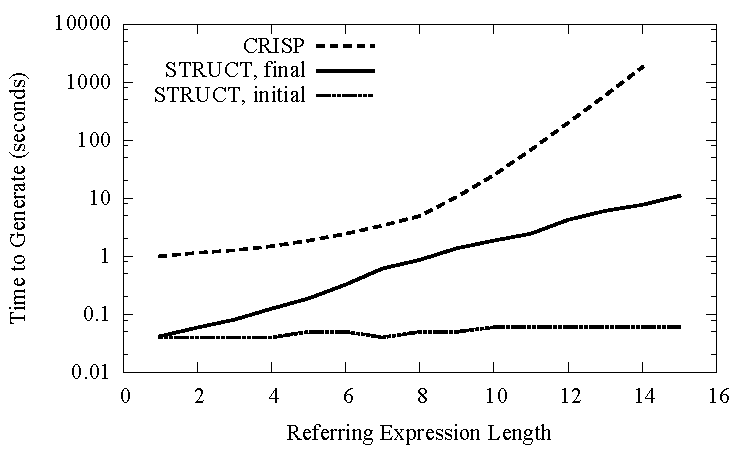
\includegraphics[width=0.7 \linewidth ]{../analysis/plots/complex-goal/complex-goal.pdf}
\caption{Experimental comparison between STRUCT and  CRISP: 
Generation time vs. length of referring expression }
\label{crisp-comparison-gentime}
\end{figure}

\begin{figure}
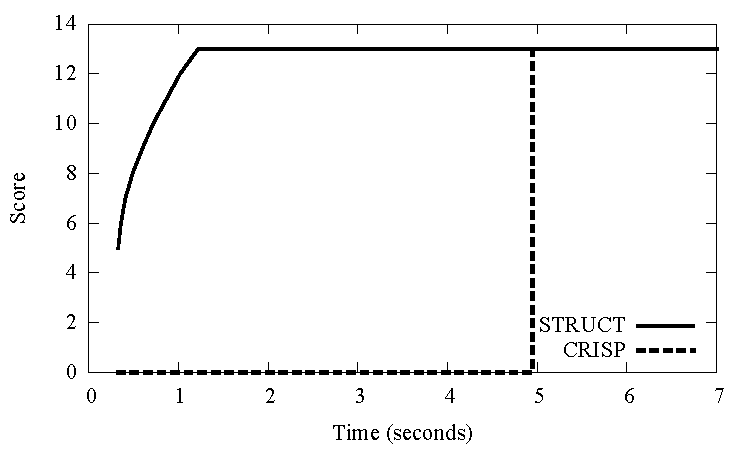
\includegraphics[width=0.7 \linewidth ]{../analysis/plots/complex-goal/complex-goal-anytime.pdf}
\caption{Experimental comparison between STRUCT and  CRISP:
Score of best solution vs time.}
\label{crisp-comparison-score}
\end{figure}

\subsection{Referring Expressions}
We first evaluate CRISP and STRUCT on their ability to generate
referring expressions. We follow prior work (\cite{koller_experiences_2011})
in our initial experiment design.  We consider a series of sentence
generation problems which require the planner to generate a sentence
like ``The Adj$_1$ Adj$_2$ ... Adj$_k$ dog chased the cat.",
where the string of adjectives is a string that distinguishes one
dog (whose identity is specified in the problem description) from
all other entities in the world.
The experiment has two parameters: $j$, the number of adjectives in
the grammar, and $k$, the number of adjectives necessary to
distinguish the entity in question from all other entities. We set $j
= k$ and show the results in Figure~\ref{crisp-comparison-gentime}.
We observe that CRISP was able to achieve
sub-second or similar times for all expressions of less than length 5, but its
generation times increase exponentially past that point, exceeding 100
seconds for some plans at length 10. At length 15, CRISP failed to
generate a referring expression; after 90 minutes the Java garbage
collector terminated the process. STRUCT$_b$, performs much better and
is able to generate much longer referring expressions without failing.
Later experiments had successful referring expression generation of lengths
as high as 25.  STRUCT$_a$ performs similarly to CRISP asymptotically.

We can also observe the anytime nature of STRUCT from this experiment,
shown in Figure~\ref{crisp-comparison-score}.  Here we look at the
length of the solution sentence generated as a function of time, for
$k=8$, a mid-range scenario which both generators are able to solve
relatively quickly ($< 5s$).  As expected, CRISP produces nothing until
the end of its run, at which point it returns the solution. STRUCT (both versions)
quickly produces a reasonable solution, ``The dog chased the
cat.''  This is then improved upon by adjoining until the referring
expression is unambiguous. If at any point the generation process was
interrupted, STRUCT would be able to return a solution that at least
partially solves the communicative goal.

\begin{figure}
\centering
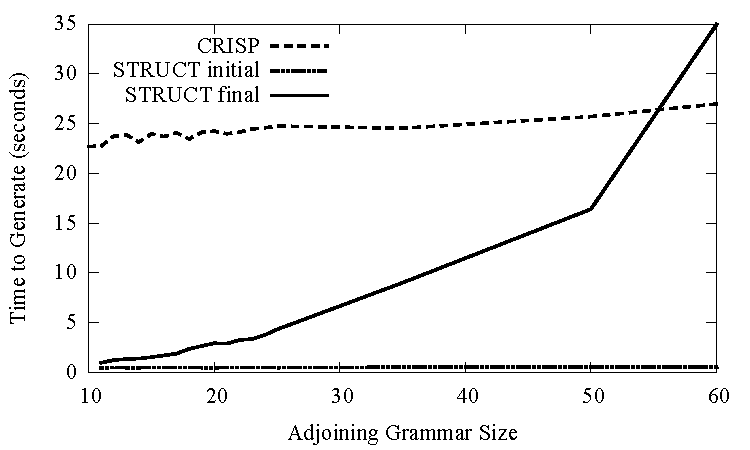
\includegraphics[width=0.7 \linewidth]{../analysis/plots/large-grammar/large-grammar.pdf}
\label{graph-large-grammars}
\caption{Effect of grammar size}
\end{figure}

\begin{figure}
\centering
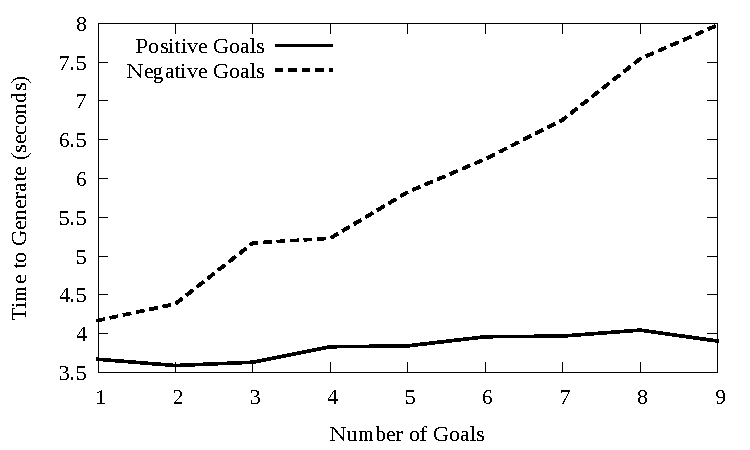
\includegraphics[width=0.7 \linewidth]{../analysis/plots/goals/differentgoals.pdf}
\label{chart-different-goals}
\caption{Effect of multiple and negated goals}
\end{figure}

\begin{figure}
\centering
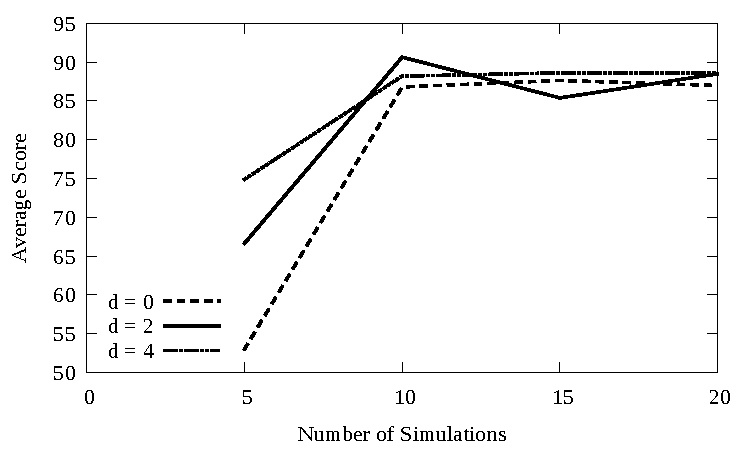
\includegraphics[width=0.7 \linewidth]{../analysis/plots/params/pltag-n-v-score.pdf}
\label{chart-n-v-score}
\caption{Effect of parameter variations on the STRUCT solution.}
\end{figure}


\subsection{Grammar Size}
We next evaluate STRUCT and CRISP's ability to
handle larger grammars. This experiment is set up in the same way as
the one above, with the exception of $l$ ``distracting'' words, words
which are not useful in the sentence to be generated.  $l$ is defined
as $j - k$.  In these experiments, we vary $l$ between 0 and 50.
Figure~\ref{graph-large-grammars} shows the results of these
experiments.  We observe that CRISP using GraphPlan, as previously
reported in \cite{koller_experiences_2011}, handles an increase in
number of unused actions very well.  Prior work reported a difference
on the order of single milliseconds moving from $j = 1$ to $j = 10$.
We report similar variations in CRISP runtime as $j$ increases from 10
to 60: runtime increases by approximately 10\% over that range.

\subsubsection{Absent Pruning}

STRUCT's performance with large grammars is similar to CRISP using the
FF planner \cite{hoffmann_ff_2001}, also profiled in
\cite{koller_experiences_2011}, which increased from 27 ms to 4.4
seconds over the interval from $j = 1$ to $j = 10$.  STRUCT's
performance is less sensitive to larger grammars than this, but over
the same interval where CRISP increases from 22 seconds of runtime to
27 seconds of runtime, STRUCT increases from 4 seconds to 32 seconds.
This is due almost entirely to the required increase in the value of
$n$ (number of samples) as the grammar size increases.  At the low
end, we can use $n=20$, but at $l = 50$, we must use $n = 160$ in
order to ensure perfect generation as soon as possible.  Fortunately,
as STRUCT is an anytime algorithm, valid sentences are available very
early in the generation process, despite the size of the set of
adjoining trees (the ``STRUCT Initial'' curve in
Figure~\ref{graph-large-grammars}).  This value does not change
substantially with increases in grammar size.  However, the time to
improve this solution does. An interesting question for future work is
how to limit this increase in time complexity in STRUCT. 

\subsubsection{With Pruning}

STRUCT's performance with large grammars improves dramatically if
we allow for pruning (described in Chapter 4).  This experiment involving distracting words
is a perfect example of a case where pruning will perform optimally.
When we apply pruning we find that STRUCT is able to completely ignore the effect of
additionaly distracting words.  Experiments showed roughly constant times for generation
for $j=1$ through $j=5000$.  Although pruning is $O(n)$ in grammar size, repeated experiments
failed to show any significant distinction in runtime, even on very large grammars.

\section{Evaluation of Complex Communicative Goals}
In the next set of experiments, we illustrate that STRUCT can solve
conjunctions of communicative goals as well as negated communicative goals.

\subsection{Multiple Goals}
We next evaluate STRUCT's ability to accomplish
multiple communicative goals when generating a single sentence.  In this
experiment, we modify the problem from the 
previous section.  In that section, the referred-to dog was unique,
and it was therefore possible to produce a referring expression which
identified it unambiguously.  In this experiment, we remove this
condition by creating a situation in which the generator will be
forced to ambiguously refer to several dogs.  We then add to the
world a number of adjectives which are common to each of these
possible referents.  Since these adjectives do not further
disambiguate their subject, our generator should not use
them in its output.  We then encode these adjectives into
communicative goals, so that they will be included in the output of
the generator despite not assisting in the accomplishment of
disambiguation.  We find that, universally, these otherwise useless
adjectives are included in the output of our generator, demonstrating
that STRUCT is successfully balancing multiple communicative goals.
As we show in figure \ref{chart-different-goals} (the ``Positive
Goals'' curve) , the presence of additional satisfiable semantic goals does
not substantially affect the time required for generation.  We are able to
accomplish this task with the same very high frequency as the CRISP
comparisons, as we use the same parameters.

\subsection{Negated Goals}
We now evaluate STRUCT's ability to generate
sentences given negated communicative goals.  We again modify
the problem used earlier by 
adding to our lexicon several new adjectives, each applicable only to
the target of our referring expression.  Since our target can now be
referred to unambiguously using only one adjective, our generator
should just select one of these new adjectives (this has been experimentally confirmed).
We then encode these
adjectives into negated communicative goals, so that they will not be
included in the output of the generator, despite allowing a much
shorter referring expression.  We find that these adjectives which
should have been selected immediately are omitted from the output, and
that the sentence generated is the best possible under the
constraints.  This demonstrates that STRUCT is balancing these negated
communicative goals with its positive goals.  Figure
\ref{chart-different-goals} (the ``Negative Goals'' curve) shows the
impact of negated goals on the time to generation.  Since this
experiment alters the grammar size, we see the time to final
generation growing linearly with grammar size.  The increased time to
generate can be traced directly to this increase in grammar size.
This is a case where pruning does not help us in reducing the grammar size;
we cannot optimistically prune out words that we do not plan to use.  Doing
so might reduce the ability of STRUCT to produce a sentence which partially
fulfills its goals.

\subsection{Nested subclauses}

Here, we evaluate STRUCT$_a$'s ability to generate sentences with nested
subclauses.  An example of such a sentence is ``The dog which ate the treat
chased the cat".  This is a difficult sentence to generate for several reasons.
The first, and clearest, is that there are words in the sentence which do not
help to increase the score assigned to the partial sentence.  Notably, we must adjoin
the word "which" to "the dog" during the portion of generation where the
sentence reads "the dog chased the cat".  This decision requires us to do planning
deeper than one level in the future, which massively increases the number of simulations
STRUCT requires in order to get the best possible result.  The second reason that
this sentence is a challenge for our generation algorithm is that that adjoinment
("the dog" $\rightarrow$ "the dog which") corresponds to a tree where the verb
that will be a child of "which" (in this case, "ate") does not have its argument as a child.
See Figure \ref{explanation-of-child} for a visual explanation of this.  Consequently,
we need to introduce indirection.  We add a node to our tree which represents the
implied subject of the verb "ate".  This is the approach taken by XTAG \cite{xtag} in
their attempt to create a TAG which appropriately represents the English language.
See Figure \ref{explanation-of-indirection} for a visual explanation.

Despite these troubles, STRUCT is capable of generating these sentences.  As we can
see in Figure \ref{nested}, STRUCT's time to generate increases with the number of
nested clauses.  To the best of our knowledge, CRISP is not able to generate sentences
of this form, and consequently we present our results without baselines.  We present
results only for STRUCT$_a$ here, since STRUCT$_b$ is not capable of generating
sentences using indirection.

\subsection{Conjunctions}

\begin{figure}
\centering
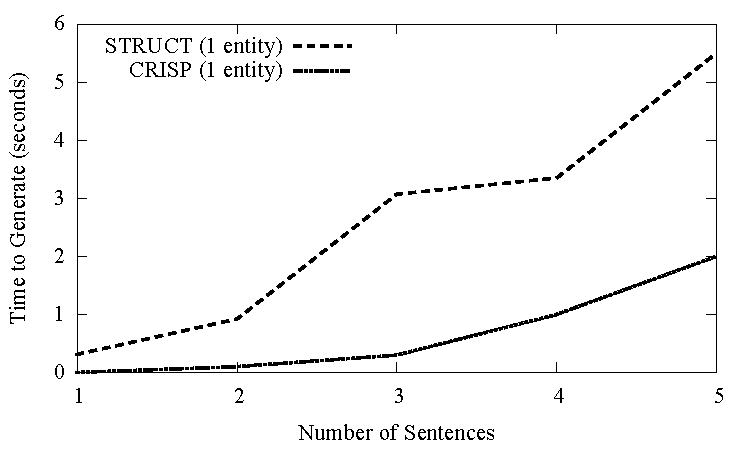
\includegraphics[width=0.7 \linewidth]{../analysis/struct/conjunction/conjunction1.pdf}
\label{graph-conjunction1}
\caption{Time to generate sentences with conjunctions with one entitiy ("The man sat and the girl sat and ....")}
\end{figure}

\begin{figure}
\centering
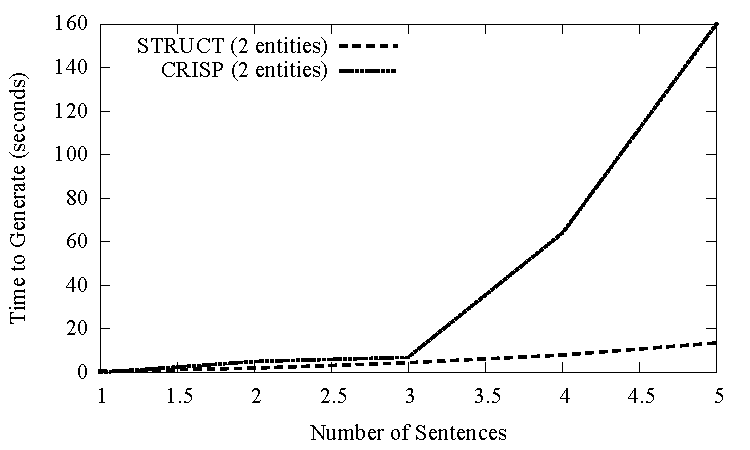
\includegraphics[width=0.7 \linewidth]{../analysis/struct/conjunction/conjunction2.pdf}
\label{graph-conjunction2}
\caption{Time to generate sentences with conjunctions with two entities ("The dog chased the cat and ...")}
\end{figure}

\begin{figure}
\centering
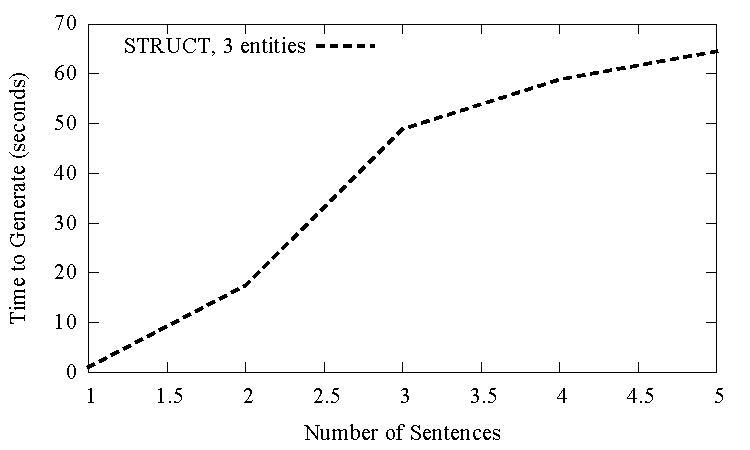
\includegraphics[width=0.7 \linewidth]{../analysis/struct/conjunction/conjunction3.pdf}
\label{graph-conjunction3}
\caption{Time to generate sentences with conjunctions with three entities ("The man gave the girl the book and ....")}
\end{figure}


Here, we evaluate STRUCT$_b$'s ability to generate sentences including
conjunctions.  We introduce the conjunction "and", which allows for the
root nonterminal of a new sentence ('S') to be adjoined to any other sentence.
We then provide STRUCT with multiple goals.  Given sufficient depth for the
search ($d=3$ was determined to be sufficient, as our reward signal is fine-grained),
STRUCT will produce two sentences joined by the conjunction "and".
Here, we follow prior work in our experiment design \cite{koller_experiences_2011}.

As we can see in Figures \ref{graph-conjunction1}, \ref{graph-conjunction2}, and
\ref{graph-conjunction3}, STRUCT successfully generates results
for conjunctions of up to five sentences.  This is not a hard upper bound, but
generation times begin to be impractically large at that point, and further
experimentation would be unnecessary.  Fortunately, human language tends toward
shorter discourse units than these unwieldy (but technically grammatical) sentences.

STRUCT increases in generation time both as the number of sentences increases and as
the number of objects per sentences increases.  We show results for STRUCT$_a$ here,
as our output should contain only simple sentences without nesting, and because
STRUCT$_b$ is exponential in number of entities in the sentence, which will cause
impractically large generation times for this experiment.

\subsection{Effect of Parameters}
Finally, we study the effect of the number of simulations and
lookahead depth on the performance of STRUCT. We design this
experiment to require lookahead by using  a sparse
reward function that penalizes a final sentence based on the number of
adjectives it has. We also use a probabilistic LTAG that has multiple
actions all relevant to reaching the goal, but that add differing
numbers of adjectives to the sentence. We then run STRUCT on this
problem with differing parameter values and report the score of the
best solution found, as measured by our reward function
(Figure~\ref{chart-n-v-score}). 

From the figure, it is clear that as the number of simulations
increase, the quality of the solution improves for all values of $d$.
This is likely because increasing simulations means a better estimate
of the utility of each action. Further, in this particular case,
increasing the depth of lookahead also yields a benefit, because of
the structure of our problem. This is especially true if the branching
factor of the search space is large, which is common in NLG
applications.  Similarly, the deeper we allow the tree search to continue, the
better the estimation of the future value of each action,
especially since actions have far-reaching consequences for the
meaning of the sentence at its conclusion. 
It is interesting that even for low numbers of
simulations $d=4$ is able able to find a reasonably good
solution. These behaviors are expected and verify 
that STRUCT does not display any pathologies with respect to its parameters.
\chapter{Conclusion and Future Work}
In conclusion, we will compare STRUCT to established NLG methods,
discuss other strengths and weaknesses of STRUCT, and describe
directions for future work.

We believe that we have produced an algorithm which unifies the
two approaches to NLG discussed in Chapter 3.  
We have fused the probabilistic reasoning and
domain knowledge use from the probabilistic ranking method with
the planning problem conversion and structured approach to semantics
from the classical planning approach.  We have the advantage of
partial goal satisfaction from ``overgenerate and rank" and the
advantage of explicit semantic meaning specification and
output from classical planning.

We have avoided the all-or-nothing weakness of classical planning,
where a classical planner cannot emit a sentence which does not
optimally satisfy the goal.  Yet, STRUCT allows generation of complex
goals, which would be intractable with a probabilistic ranking generator.
We have avoided the requirement that we specify a large percentage of
our output as input, which is a problem with probabilistic ranking.

In short, we have constructed an algorithm with many of the strengths
of both classical planning and probabilistic ranking, and few of the
weaknesses of either.

STRUCT's prime strength is its ability to partially satisfy goals in cases where
perfectly correct generation is impossible, either because of conflicting
goals or because of a grammar which does not allow for all goals.
This allows STRUCT to be used in situations even without perfect knowledge
of the domain, since STRUCT can recover from some of the issues that come
from unknown domains (like a grammar which is too small or insufficient knowledge
of the world), and continue attempting to generate close-to-optimal output
where other generators would either fail after churning on the problem
for a long time, or emit something nonsensical.

Another important strength of STRUCT is its anytime nature; something which
we have not seen done before.  STRUCT is capable of creating an approximate
solution very quickly (usually less than 0.5 seconds), and that approximate solution
can be emitted if the user desires a response very quickly.  The solution will be iteratively
improved until it reaches a sentence which fulfills all communicative goals given.

One important weakness of STRUCT is the rapid increase in generation time
past certain limits.  STRUCT has trouble generating referring expressions of
length 10 or more, and has trouble generating sentences which adjoin
more than about 5 verbs.

STRUCT also is limited by its grammar.  It is difficult to produce an LTAG grammar
for English, and any such grammar will, by nature, overgenerate (the language
specified by the grammar will contain some constructs not acceptable in
English).  It is best to build a grammar which undergenerates (the language
specified by the grammar is a subset of acceptable English), but that can
be difficult without knowledge of which constructs exactly will be necessary.

Due to some peculiarities of the python interpreter, we were unable to
efficiently parallelize UCT during the search phase of generation.  This
would be relatively straightforward using a worker pool solution, and we
could drastically shrink the amount of time spent in that search.

We may also be able to use STRUCT as the output generator of a dialog system,
similar to NJFun \cite{litman_njfun_2000}, instead of the template-based generation
that most such systems employ.  STRUCT would be substantially more flexible in
its output than a template-based system, which can usually only respond to preprogrammed
error cases.  STRUCT's ability to partially accomplish communicative goals would be
valuable in this application.

We are also interested in reward functions.  The reward functions we have created
are good for generating language based on facts about the world, and would
serve for goal-directed communication, but those are not the only possible
goals of natural language generation.  If we could learn a reward function from
a corpus and attempt to emulate that corpus in our speech, or build a hierarchical
reward function which could attempt to accomplish secondary or tertiary goals
in addition to a primary one.  We should explore the possibilities that the
generality of our architecture afford us.

In conclusion, we have presented an algorithm which performs Natural Language
Generation in a well-principled way, unifying two popular schools of thought regarding
NLG.  Experimental evaluation shows that it performs as well as the state-of-the-art in
the field, and its nature allows for a substantially greater set of use cases than either
of the popular schools it synthesizes.

% appendix
%\begin{appendices}               % Start of the Appendix Chapters.  If there is only
                                 % one Appendix Chapter, then use \begin{appendix}
\begin{appendix}
\chapter{Example Grammars}
\section{Basic Experiment}

\begin{figure}[h]
\caption{Grammar for the basic experiment}
\begin{lstlisting}
"grammar" :
{
    "i.nvn":    "(S(NP-subj)(VP(V+-self)(NP-obj)))",
    "i.np":     "(NP(D)(N+-self))",
    "i.d":      "(D+-self)",
    "i.cv":     "(V+-self)",
    "a.ad":     "(N(A+)(N*-self))",
    "a.sub":    "(N(N*-self)(PP(P+-clause)(VP(V-clauseverb|self,clauseobj)(NP-clauseobj))))"
}
\end{lstlisting}
\end{figure}

\begin{figure}[h]
\caption{Lexicon for the basic experiment}
\begin{lstlisting}
"lexicon":
{
    "i.nvn": [{"word" : "chased", "meaning": "chased(subj, obj)"}, {"word":"ate", "meaning":"ate(subj, obj)"}],
    "i.d":  [{"word":"the","meaning": None}, {"word":"a", "meaning":None}],
    "i.np":   [{"word":"cat", "meaning":"cat(self)"}, {"word":"dog", "meaning":"dog(self)"}, 
    {"word":"treat", "meaning":"treat(self)"}],
    "a.ad":  [],
    "i.cv": [{"word":"chased", "meaning":"chased(self)"}],
    "a.sub": [{"word":"which", "meaning":None}]
}
\end{lstlisting}
\end{figure}

\begin{figure}[h]
\caption{World and Goal for the basic experiment}
\begin{lstlisting}
{
    "world": ["chased(d1, c)", "dog(d1)", "cat(c)"],
    "goal": "chased(d1, c)"
}
\end{lstlisting}
\end{figure}

\begin{figure}[h]
\caption{Example input for Halogen; appears in \cite{knight_1995_genselect}}
\begin{lstlisting}
(A / Ihave the quality of beingl 
:DOMAIN (P / [procurel 
:AGENT (A2 / [American[) 
:PATIENT (G / [gun, arml)) 
:RANGE (E / [easy, effortless[)) 
\end{lstlisting}
\label{halogen-example}
\end{figure}
\end{appendix}
%\include{app2_workspace}
%\include{app3_r2}
%\include{code}                   % Including computer code listings
%\include{bibref}                 % a BibTeX reference
%\include{math}                   % Complex Equations from the UW Math Department
%\include{acro}                   % A discussion on generating PDF files.
%\end{appendices}                 % End of the Appendix Chapters.  ibid on \end{appendix}

\bibliography{thesis_ref}              % Make the bibliography

%\include{vita}                  % Optional Vita, use \begin{vita} vita text \end{vita}
\end{document}

